% !TEX root = task-26.tex
% EGE 2027, task 26. Source IDs and URLs are kept in comments.
% Editable task bank. Append new BankTask blocks at the end of the document.
\documentclass[12pt,a4paper]{article}
\usepackage{physics-textbook}
\usepackage{graphicx,needspace}
\usetikzlibrary{decorations.pathmorphing}
\newif\ifShowSolutions
\ifdefined\TutorEdition
  \ShowSolutionstrue
\else
  \ShowSolutionsfalse % Change to \ShowSolutionstrue to display solutions.
\fi
\newcounter{banktask}
\newsavebox{\BankTaskBox}
\newcommand{\BankTaskContent}[3]{%
  \noindent\textbf{\thebanktask.}\quad #2\par
  \ifShowSolutions
    \Needspace{50mm}% Keep the solution heading with its opening text or diagram.
    #3\par
    \ifdefined\TutorEdition
      \ifcsname TutorSource#1\endcsname
        \nopagebreak\smallskip{\small\csname TutorSource#1\endcsname\par}%
      \fi
    \fi
  \fi
}
\newcommand{\BankTask}[3]{%
  \refstepcounter{banktask}\par\medskip
  \sbox{\BankTaskBox}{\begin{minipage}{\linewidth}%
    \BankTaskContent{#1}{#2}{#3}\end{minipage}}%
  \ifdim\dimexpr\ht\BankTaskBox+\dp\BankTaskBox\relax>\dimexpr\textheight-20mm\relax
    \Needspace{35mm}\BankTaskContent{#1}{#2}{#3}%
  \else
    \Needspace{\dimexpr\ht\BankTaskBox+\dp\BankTaskBox\relax}%
    \noindent\usebox{\BankTaskBox}\par
  \fi
  \medskip
}
\begin{document}


% Source 42654: https://phys-ege.sdamgia.ru/problem?id=42654
\BankTask{42654}{
\begin{center}\begin{tikzpicture}[task graph,>=stealth]
\draw(-.3,0)--(3,0)--(3,-.8);
\foreach \x in {0,.2,...,2.8}{\draw(\x,0)--++(-.12,-.12);}
\draw[fill=white](0,0)rectangle(4,.18);
\node[above left]at(0,.18){$A$};\node[right]at(4,.18){$B$};\node[above]at(2,.18){$M$};
\draw(4,.18)--(4,2.5);\draw(4.6,2.5)circle(.6)(4.6,2.5)circle(1.2);
\draw(5.8,2.5)--(5.8,-.4);\draw[fill=white](5.5,-1)rectangle(6.1,-.4);\node at(5.8,-.7){$m$};
\draw[fill=white](4.23,4)--(4.52,2.48)--(4.68,2.48)--(4.97,4)--cycle;\node at(4.6,2.64){$\times$};\draw(3.55,4)--(5.65,4);
\foreach \x in {3.6,3.8,...,5.6}{\draw(\x,4)--++(.12,.12);}
\node[left]at(3.4,2.5){$R$};\node at(4.65,2.1){$r$};
\end{tikzpicture}\end{center}Однородный брусок $AB$ массой $M$ постоянного прямоугольного сечения лежит на гладкой горизонтальной поверхности стола, свешиваясь с него менее чем наполовину (см. рисунок). К правому концу бруска прикреплена легкая нерастяжимая нить. Другой конец нити закреплен на меньшем из двух дисков идеального составного блока. На большем диске этого блока закреплена другая легкая нерастяжимая нить, на которой висит груз массой $m$. Диски скреплены друг с другом, образуя единое целое, где $R$  =  $10\,\text{см}$, $r$  =  $5\,\text{см}$.
Сделайте рисунок с указанием сил, действующих на брусок $M$, блок и груз $m$. Найдите максимальное значение дроби  $\frac{m}{M} ,$ при котором система тел остается неподвижной. Трением в оси блока пренебречь. Обоснуйте применимость используемых законов к решению задачи.
}{
\smallskip\noindent\textbf{Решение}\par
Обоснование. 
$1$.  Систему отсчета, связанную с Землей, будем считать инерциальной (ИСО). 
$2$.  Брусок перед отрывом его правого края от поверхности стола будем считать твердым телом с осью вращения, проходящей перпендикулярно плоскости рисунка через точку $A$. Условие равновесия относительно вращения твердого тела на оси  — равенство нулю суммы моментов сил, приложенных к телу, относительно этой оси. 
$3$.  Нити нерастяжимы, поэтому, если покоится брусок, то покоятся и все остальные тела системы. $4$. Нити легкие, поэтому величина силы натяжения каждой нити в любой ее точке одна и та же. В том числе: $T_1=T_3,$ $T_2=T_4$ (см. рис. в решении). 
$5$.  Блок идеальный (трения в осях нет, масса блока пренебрежимо мала). Поэтому условие равновесия блока  — равенство нулю суммы моментов сил натяжения нитей относительно оси блока. 
$6$.  Груз может двигаться только поступательно вдоль вертикальной оси $Oy$, лежащей в плоскости рисунка. Поэтому для груза используем модель материальной точки и применим второй закон Ньютона. Вследствие этого условие равновесия - сумма приложенных к грузу сил равна нулю.
Решение.\begin{center}\begin{tikzpicture}[task graph,>=stealth]\draw(-.3,0)--(3,0)--(3,-.7);\draw[very thick](0,.08)--(3.8,.08);\node[above left]at(0,.08){$A$};\node[right]at(3.8,.08){$B$};\draw(3.8,.08)--(3.8,2);\draw(4.3,2)circle(.5)(4.3,2)circle(.8);\draw(5.1,2)--(5.1,-.6);\draw[fill=gray!15](4.9,-.9)rectangle(5.3,-.5);\draw[fill=white](4.07,3.2)--(4.22,1.94)--(4.38,1.94)--(4.53,3.2)--cycle;\draw(3.45,3.2)--(5.15,3.2);\draw[->](-.4,0)--(6,0)node[right]{$x$};\draw[->](.7,-1.2)--(.7,1.6)node[above]{$y$};\node[below left]at(.7,0){$O$};\draw[->,thick](0,.08)--(0,.9)node[above left]{$\vec N$};\draw[->,thick](1.9,.08)--(1.9,-1.1)node[right]{$M\vec g$};\draw[->,thick](3.8,.08)--(3.8,.85)node[left]{$\vec T_1$};\draw[->,thick](3.8,2)--(3.8,1.35)node[left]{$\vec T_3$};\draw[->,thick](5.1,2)--(5.1,1.15)node[right]{$\vec T_4$};\draw[->,thick](4.3,2)--(4.3,3.6)node[above]{$\vec F$};\draw[->,thick](5.1,-.5)--(5.1,.35)node[right]{$\vec T_2$};\draw[->,thick](5.1,-.9)--(5.1,-1.6)node[right]{$m\vec g$};\end{tikzpicture}\end{center}
$1$.  Силы, действующие на брусок, блок и груз, показаны на рисунке для случая, когда масса бруска минимальна, и поэтому он еще покоится на столе, но касается стола только в точке $A$. Поэтому сила $\vec N$ приложена к бруску в точке $A$ и направлена вертикально вверх, так как поверхность стола гладкая (трения нет). 
$2$.  Запишем уравнение моментов сил для бруска в момент, когда он покоится, касаясь стола только в точке $A$: 

\[T_1 \cdot A B - M g \cdot \frac{A B}{2} =0,\]

 откуда 

\[T_1= \frac{M g}{2} .\]

$3$.  Запишем второй закон Ньютона для покоящегося груза в проекциях на ось Оу введенной ИСО: $T_2 - m g=0,$ откуда $T_2=m g.$ 
$4$.  Условие равновесия блока на его оси: $T_3 \cdot r=T_4 \cdot R .$ С учетом того, что $T_1=T_3$ и $T_2=T_4,$ получим отсюда $T_1 \cdot r=T_2 \cdot R .$
$5$.  Подставив в это равенство результаты п. $2$ и $3$, получим: 

\[\frac{M g}{2} \cdot r=m g \cdot R.\]

Искомое отношение будет максимальным, если масса $M$ будет минимальной. Найдем это отношение:

\[\frac{m}{M} = \frac{r}{2R} = \frac{5}{2 \cdot 10} =0{,}25.\]

Ответ: $0{,}25$.
}

% Source 25744: https://phys-ege.sdamgia.ru/problem?id=25744
\BankTask{25744}{
Два небольших шара массами $m_{1}$ = $0{,}2\,\text{кг}$ и $m_{2}$ = $0{,}3\,\text{кг}$ закреплены на концах невесомого стержня $AB$, расположенного горизонтально на опорах $C$ и $D$ (см. рис.). Расстояние между опорами l = $0{,}6\,\text{м}$, а расстояние $AC$ равно $0{,}2\,\text{м}$. Чему равна длина стержня $L$, если сила давления стержня на опору $D$ в $2$ раза больше, чем на опору $C$? Сделайте рисунок с указанием внешних сил, действующих на систему тел «стержень  — шары».
Какие законы Вы используете для описания равновесия тела? Обоснуйте их применение к данному случаю.
\begin{center}\begin{tikzpicture}[task graph,>=stealth]
\draw(.5,1)rectangle(5.5,1.15);\draw(.5,.75)circle(.25)(5.5,.75)circle(.25);
\node[above]at(.5,1.15){$A$};\node[above]at(5.5,1.15){$B$};
\node[left]at(.25,.65){$m_1$};\node[right]at(5.75,.65){$m_2$};
\draw(1.8,0)--(2,1)--(2.2,0)--cycle;\draw(4.5,0)--(4.7,1)--(4.9,0)--cycle;
\node[left]at(2,.8){$C$};\node[left]at(4.7,.8){$D$};\draw(.2,0)--(5.8,0);
\foreach \x in {.4,.6,...,5.8}{\draw(\x,0)--++(-.12,-.12);}
\end{tikzpicture}\end{center}
}{
\smallskip\noindent\textbf{Решение}\par
Обоснование. Систему отчета, связанную с Землей, будем считать инерциальной. Для данной системы отсчета можно применить законы Ньютона (в частности, третий закон).
Тело, образованное стержнем и двумя шарами, будем считать абсолютно твердыми. Движение абсолютно твердого тела представляет собой суперпозицию поступательного и вращательного движений, поэтому для него можно применить условие равновесия для поступательного движения и правило моментов. Векторная сумма всех внешних сил, действующих на тело, равна нулю, поэтому сумма моментов этих сил относительно двух любых его параллельных осей одна и таже. Для удобства ось, относительно которой будем рассматривать сумму моментов сил, проведем перпендикулярно плоскости чертежа через точку А.

Перейдем к решению. На твердое тело, образованное стержнем и двумя шарами, действуют силы тяжести $m_1\vec g$ и $m_2\vec g,$ приложенные к центрам шаров, и силы реакции опор $\vec N_1$ и $\vec N_2.$ По третьему закону Ньютона, модули сил реакции равны соответствующим модулям сил давления стержня на опоры, поэтому $N_2 = 2N_1$ (в соответствии с условием задачи).
\begin{center}\begin{tikzpicture}[task graph,>=stealth]\draw[->](-.6,-.5)--(6,-.5)node[right]{$x$};\foreach \xx in {-.6,-.44,...,5.45}{\draw(\xx,-.5)--++(.12,-.12);}\draw[->](-.6,-1.8)--(-.6,2.1)node[above]{$y$};\node[below left]at(-.6,-.5){$O$};\draw[fill=gray!10](0,.55)rectangle(5,.7);\foreach\x/\l in{0/A,5/B}{\draw[fill=gray!15](\x,.3)circle(.2);\node[above]at(\x,.85){$\l$};}\foreach\x/\l in{1.4/C,4.2/D}{\draw(\x,.55)--++(-.2,-1.05)--++(.4,0)--cycle;\node[left]at(\x,.1){$\l$};}\node[right]at(.3,.2){$m_1$};\node[right]at(5.3,.2){$m_2$};\draw[->,thick](1.4,.55)--(1.4,1.6)node[above]{$\vec N_1$};\draw[->,thick](4.2,.55)--(4.2,2)node[above]{$\vec N_2$};\draw[->,thick](0,.3)--(0,-1.4)node[right]{$m_1\vec g$};\draw[->,thick](5,.3)--(5,-1.6)node[right]{$m_2\vec g$};\end{tikzpicture}\end{center}
В инерциальной системе отсчета $Oxy$, связанной с Землей, условия равновесия твердого тела приводят к набору уравнений:

\[N_1 + N_2 - m_1g - m_2g = 0\]

  — центр масс не движется вдоль оси $Oy$.

\[N_1x + N_2 ( l + x ) - m_2gL = 0\]

  — нет вращения вокруг оси, проходящей перпендикулярно рисунку через точку $A$.
 Здесь $x = AC = 0{,}2\,\text{м}$  — плечо силы реакции $N_{1}$.
 С учетом условия $N_2 = 2N_1$ уравнения приводятся к виду:

$3N_1 = ( m_1 + m_2 ) g,$
$( 3x + 2l ) N_1 = m_2gL.$

 Поделив второе уравнение на первое, получим:

\[L \frac{m_2}{m_1 + m_2} = x + \frac{2}{3} l.\]

 Откуда:

\[L = ( 1 + \frac{m_1}{m_2} ) \cdot ( x + \frac{2}{3} l ) = ( 1 + \frac{0{,}2\,\text{кг}}{0{,}3\,\text{кг}} ) \cdot ( 0{,}2\,\text{м} + \frac{2}{3} \cdot 0{,}6\,\text{м} ) = 1\,\text{м}.\]

Ответ: $1\,\text{м}$.
}

% Source 35160: https://phys-ege.sdamgia.ru/problem?id=35160
\BankTask{35160}{
Шар массой $1\,\text{кг}$, подвешенный на нити длиной $90\,\text{см}$, отводят от положения равновесия на угол $60$° и отпускают. В момент прохождения шаром положения равновесия в него попадает пуля массой $10\,\text{г}$, летящая навстречу шару. Она пробивает его и продолжает двигаться горизонтально. Определите модуль изменения импульса пули в результате попадания в шар, если он, продолжая движение в прежнем направлении, отклоняется на угол $39$°. (Массу шара считать неизменной, диаметр шара  — пренебрежимо малым по сравнению с длиной нити, $\cos 39 ^\circ = \frac{7}{9} .$) Какие законы Вы используете для решения задачи? Обоснуйте их применение.
}{
\smallskip\noindent\textbf{Решение}\par
Обоснование
$1$.  Введем инерциальную систему отсчета (ИСО), связанную с Землей.
$2$.  Тела движутся поступательно, размеры шарика малы по сравнению с размером нити, поэтому шарик и пулю можно описывать моделью материальной точки.
$3$.  Будем считать время взаимодействия пули и шарика малым, чтобы нить за время соударения не успела заметно отклониться. Тогда все силы в момент соударения направлены вертикально. Следовательно, в ИСО при попадании пули в шарик сохраняется горизонтальная составляющая импульса системы «шарик + пуля».
$4$.  После попадания пули в шарик при движении тел по вертикальной окружности механическая энергия равна сумме кинетической и потенциальной энергий тел $E=E_{\,\text{п}} + E_{\,\text{к}}.$ Изменение механической энергии тел в ИСО равно работе всех непотенциальных сил, приложенных к телу. Работа непотенциальной силы натяжения нити равна нулю, так как сила натяжения направлена перпендикулярно скорости в любой точке траектории.
$5$.  За нулевой уровень потенциальной энергии примем уровень положения равновесия шарика.

Перейдем к решению.
Потенциальная энергия равна $E_{\,\text{п}}=Mgh=Mgl ( 1 - \cos \alpha ) .$
Кинетическая энергия шарика в нижней точке $E_{\,\text{к}}= \frac{M v _0 ^2}{2} .$
По закону сохранения энергии:

\[Mgl ( 1 - \cos \alpha ) = \frac{M v _0 ^2}{2} .\]

Тогда скорость шарика в нижней точке равна:

\[v _0= \sqrt{2gl ( 1 - \cos \alpha )} .\]

Запишем законы сохранения импульса в момент удара и закон сохранения энергии после удара и до подъема шарика на максимальную высоту:

\[\begin{cases}Mv_0-mv_1=Mu-mv_2,\\ \dfrac{Mu^2}{2}=Mgl(1-\cos\beta).\end{cases}\]

Находим скорость шарика сразу после удара:

\[u= \sqrt{2gl ( 1 - \cos \beta )} .\]

Тогда изменение скорости пули равно:

$|\Delta v | = v _1 - v _2= \frac{M \sqrt{2gl}}{m} ( \sqrt{1 - \cos \alpha} - \sqrt{1 - \cos \beta} ) ;$
$|\Delta v|=\frac{1\cdot\sqrt{2\cdot10\cdot0{,}9}}{0{,}01}\left(\sqrt{1-0{,}5}-\sqrt{1-\frac79}\right)=100\,\text{м/с}.$

Модуль изменения импульса пули равен:

\[|\Delta p|=m|\Delta v |=0{,}01 \cdot 100=1 \,\text{кг} \cdot \,\text{м/с} .\]

Ответ: $1 \,\text{кг} \cdot \,\text{м/с} .$
}

% Source 39272: https://phys-ege.sdamgia.ru/problem?id=39272
\BankTask{39272}{
Пластилиновый шарик в момент t  =  $0$ бросают с горизонтальной поверхности Земли под углом $\alpha$ к горизонту. Одновременно с некоторой высоты над поверхностью Земли начинает падать из состояния покоя другой такой же шарик. Шарики абсолютно неупруго сталкиваются в воздухе. Сразу после столкновения скорость шариков направлена горизонтально. Время от столкновения шариков до их падения на Землю равно $\tau$. С какой начальной скоростью $\upsilon_{0}$ был брошен первый шарик? Сопротивлением воздуха пренебречь.
}{
\smallskip\noindent\textbf{Решение}\par
\begin{center}\begin{tikzpicture}[task graph,>=stealth]\draw[->](0,0)--(8.8,0)node[right]{$x$};\draw[->](0,0)--(0,4.8)node[above]{$y$};\node[below left]at(0,0){$0$};\draw[domain=0:8.4,samples=60]plot(\x,{1.333333*\x-.15873016*\x*\x});\draw[->](0,0)--(.8,1.066667)node[above left]{$\vec v_0$};\draw(.6,0)arc(0:53.1301:.6)node[midway,right]{$\alpha$};\coordinate(B)at(2.1,2.1);\coordinate(A)at(2.1,3.4);\fill(B)circle(1.7pt)node[left]{$B$};\fill(A)circle(1.7pt)node[left]{$A$};\draw(A)--(B);\draw[->,thick](B)--(3.8,3.233333)node[above]{$m\vec v_1$};\draw[->,thick](B)--(3.8,2.1)node[right]{$2m\vec u_0$};\draw[->,thick](B)--(2.1,.966667)node[right]{$m\vec v_2$};\draw[dashed](3.8,3.233333)--(3.8,2.1);\draw[dashed](2.1,.966667)--(3.8,2.1);\end{tikzpicture}\end{center}Обоснование.
$1$.  Выберем инерциальную систему отсчёта, связанную с Землёй. За начало отсчёта координат примем первоначальное положение первого шарика.
$2$.  Шарики будем считать материальными точками.
$3$.  Так как сопротивлением воздуха можно пренебречь, то движение шариков можно считать свободным падением.
$4$.  Считаем время взаимодействия шариков при неупругом столкновении малым. Следовательно, импульсом внешней силы (силы тяжести) за это время можно пренебречь. Значит, импульс системы двух шариков при столкновении сохраняется. 

Перейдем к решению.
$1$.  Первый шарик начинает движение из начала координат, а второй  — из точки $A$. До и после столкновения, происходящего в точке $B$, шарики свободно падают. Следовательно, до столкновения для первого шарика

$y_1 ( t ) = v _0y t - \frac{gt ^2}{2} = v _0 \sin \alpha \cdot t - \frac{gt ^2}{2} ,$ 
$v _1y ( t ) = v _0 \sin \alpha - gt,$

а для второго шарика $v _2y ( t ) = - gt.$
$2$.  Шарики сталкиваются в момент $t_{1}$, при этом импульс системы двух шариков сохраняется: $m \vec v _1 + m \vec v _2 = 2m \vec u_0,$ а скорость $\vec u_0$ шариков после удара согласно условию горизонтальна. Следовательно,

\[v _1y ( t_1 ) + v _2y ( t_1 ) = 0 \Longleftrightarrow ( v _0 \sin \alpha - gt_1 ) + ( - gt_1 ) = 0 \Longleftrightarrow t_1 = \frac{v _0 \sin \alpha}{2g} .\]

$3$.  Столкновение шариков происходит на высоте

\[h = y_1 ( t_1 ) = v _0 \sin \alpha \cdot t_1 - \frac{gt_1 ^2}{2} = \frac{v _0 ^2 \sin ^2 \alpha}{2g} - \frac{v _0 ^2 \sin ^2 \alpha}{8g} = \frac{3}{8} \cdot \frac{v _0 ^2 \sin ^2 \alpha}{g} .\]

$4$.  Скорость $\vec u_0$ шариков после удара горизонтальна, поэтому интервал времени $\tau$ от столкновения шариков до их падения на Землю находится из условия $h = \frac{g \tau ^2}{2} ,$ откуда $\tau = \sqrt{\frac{2h}{g}} = \sqrt{3} \cdot \frac{v _0 \sin \alpha}{2g} .$ Таким образом, $v _0 = \frac{2g \tau}{\sqrt{3} \sin \alpha} .$

Ответ: $v _0 = \frac{2g \tau}{\sqrt{3} \sin \alpha} .$
}

% Source 25774: https://phys-ege.sdamgia.ru/problem?id=25774
\BankTask{25774}{
Имеется недеформированная пружина длиной $L$  =  $30\,\text{см}$ и жесткостью $k$  =  $30\,\text{Н/м}$, груз массой $m$  =  $1\,\text{кг}$, а также вращающийся с частотой $\nu = 0{,}5\,\text{Гц}$ массивный диск. На каком минимальном расстоянии от центра диска можно положить на него груз, прикрепив его пружиной к центру диска, чтобы груз оставался неподвижным относительно диска? Коэффициент трения между грузом и диском $\mu=0{,}5.$ Размерами груза пренебречь. Сделайте схематический рисунок с указанием сил, действующих на груз.
Какие законы Вы использовали для описания движения бруска? Обоснуйте их применимость к данному случаю.
}{
\smallskip\noindent\textbf{Решение}\par
Обоснование. 
$1$.  Рассмотрим задачу в инерциальной системе отсчета, связанной с Землей. Будем считать эту систему отсчета инерциальной (ИСО). Тело описываем моделью материальной точки, так как его размеры малы по сравнению с диском. 
$2$.  При вращении диска на тело действуют потенциальная сила тяжести, сила реакции опоры, перпендикулярная опоре, потенциальная сила упругости, возникающая в упруго деформированной пружине и сила трения покоя. Работа силы тяжести и силы реакции опоры равны нулю. 
$3$.  Поскольку тело описывается моделью материальной точки, в ИСО применим второй закон Ньютона. Равнодействующая сила направлена к центру, следовательно, тело движется с центростремительным ускорением. Для материальной точки применимы законы равномерного движения по окружности.
$4$.  При малых деформациях их можно считать упругими, поэтому для пружины верен закон Гука.
$5$.  Брусок покоится относительно диска, имеющего шероховатую поверхность. Поэтому на него действует максимальная сила трения покоя, равная силе трения скольжения $F_{\,\text{тр}}=\mu N.$

Перейдем к решению. \begin{center}\begin{tikzpicture}[task graph,>=stealth]\draw(.1,0)--(5,0)--(5,-.4)--(.1,-.4);\draw[dashed](.1,0)--(-.85,0)--(-.85,-.4)--(.1,-.4);\draw(-.4,-.4)--(.1,-.4)--(.1,1.8);\draw[very thick](.1,-.4)--(.1,1.8);\draw[fill=gray!15](3,.05)rectangle(4.2,.85);\draw(.1,.45)--(.3,.45);\draw plot[domain=0:1,samples=100]({.3+2.7*\x},{.45+.15*sin(2880*\x)});\node[below right]at(5.2,-1.1){$O$};\draw[->](5.2,-1.1)--(5.2,2.1)node[above]{$y$};\draw[->](5.2,-1.1)--(1.2,-1.1)node[left]{$x$};\draw[->](.1,1.8)..controls(-.5,2.3)and(.6,2.3)..(.1,1.8)node[above left]{$\nu$};\draw[->,thick](3.6,.45)--(3.6,2.3)node[above]{$\vec N$};\draw[->,thick](3.6,.45)--(3.6,-.9)node[right]{$m\vec g$};\draw[->,thick](3.6,.45)--(5,.45)node[right]{$\vec F_{\text{упр}}$};\draw[->,thick](3.6,.45)--(1.9,.45)node[above left]{$\vec F_{\text{тр}}$};\draw[->,thick](2.6,2.3)--(1.4,2.3)node[above left]{$\vec a_{\text{ц}}$};\end{tikzpicture}\end{center} 
$1$.  На груз действуют четыре силы: сила тяжести $m\vec g,$ нормальная составляющая силы реакции опоры $\overrightarrow{N},$ сила упругости $\overrightarrow{F}_{\,\text{упр}}$ и сила трения $\overrightarrow{F}_{\,\text{тр}}.$
Выясним, в каком состоянии будет находиться пружина. Если грузик находится на расстоянии $L$ от центра, то равнодействующая сила равна $ma=4 \pi ^2 \nu ^2 Lm=3$$H$. Максимальная сила трения равна $F_{\,\text{т}} =\mu mg =5$$H$. Значит, пружина должна быть сжата, сила упругости направлена вправо (см. рис.), а сила трения  — влево. Поскольку пружина максимально сжата, а груз при этом находится в покое относительно диска, сила трения покоя принимает максимальное значение: $F_{\,\text{тр}}=\mu N.$
$2$.  Второй закон Ньютона в проекциях на оси инерциальной системы отсчета XOY имеет вид: $OX: ma_{\,\text{ц}}=F_{\,\text{тр}} - F_{\,\text{упр}};$ $OY: 0=N - mg.$ Сила упругости определяется законом Гука: $F_{\,\text{упр}}=k\Delta x.$ Центростремительное ускорение груза выражается формулой $a_{\,\text{ц}}= \frac{V ^2}{R_{\min}} =4 \pi ^2 \nu ^2 R_{\min}.$
$3$.  Из формул, приведенных выше, получаем: $4 \pi ^2 \nu ^2 R_{\min}m=\mu mg - k\Delta x,$ где $R_{\min}=L - \Delta x.$ Окончательно получим:

\[R_{\min}= \frac{kL - \mu mg}{k - 4 \pi ^2 \nu ^2 m} = \frac{30 \cdot 0{,}3 - 0{,}5 \cdot 1 \cdot 10}{30 - 4 \cdot 3{,}14 ^2 \cdot 0{,}5 ^2 \cdot 1} \approx 0{,}2 \,\text{м}.\]

Ответ: $R_{\min}\approx 0{,}2 \,\text{м}.$
}

% Source 25407: https://phys-ege.sdamgia.ru/problem?id=25407
\BankTask{25407}{
\begin{center}\begin{tikzpicture}[task graph,>=stealth]
\draw(0,3.5)--(4,3.5);\foreach \x in {0,.2,...,4}{\draw(\x,3.5)--++(.12,.12);}
\draw[decorate,decoration={zigzag,segment length=4mm,amplitude=1.4mm}](.4,3.4)--(.4,1.6);
\draw[decorate,decoration={zigzag,segment length=4mm,amplitude=1.4mm}](3.6,3.4)--(3.6,1.6);
\draw(.4,3.5)--(.4,3.4)(3.6,3.5)--(3.6,3.4)(.4,1.6)--(.4,1.5)(3.6,1.6)--(3.6,1.5);
\draw(.2,1.3)rectangle(3.8,1.5);\draw(3,1.3)--(3,.8);\draw(2.7,.2)rectangle(3.3,.8);
\end{tikzpicture}\end{center}К двум вертикально расположенным пружинам одинаковой длины подвесили однородный стержень длиной $L=30\,\text{см}.$ Если к этому стержню подвесить груз массой $m=3\,\text{кг}$ на расстоянии $d=5\,\text{см}$ от правой пружины, то стержень будет расположен горизонтально, и растяжения обеих пружин будут одинаковы (см. рис.). Жесткость левой пружины в $2$ раза меньше, чем правой. Чему равна масса стержня $M$? Сделайте рисунок с указанием используемых в решении сил.
Какие законы Вы использовали для описания равновесия системы? Обоснуйте их применимость к данному случаю.
}{
\smallskip\noindent\textbf{Решение}\par
Обоснование
$1$.  Рассмотрим задачу в системе отсчета, связанной с Землей. Будем считать эту систему отсчета инерциальной (ИСО).
$2$.  Описываем стержень моделью твердого тела (формы и размеры тела неизменны, расстояние между любыми двумя точками тела остается неизменным).
$3$.  Любое движение твердого тела является суперпозицией поступательного и вращательного движений. Поэтому условий равновесия твердого тела в ИСО ровно два: одно для поступательного движения, другое - для вращательного движения.
$4$.  Сумма приложенных к твердому телу внешних сил равна нулю (условие равновесия твердого тела относительно поступательного движения). Поэтому сумма моментов этих сил относительно любых двух параллельных осей одна и та же. Для удобства выберем ось, проходящую перпендикулярно плоскости рисунка через центр масс стержня (точку О).
Решение
\begin{center}\begin{tikzpicture}[task graph,>=stealth]\draw(-.3,3)--(5.3,3);\draw(0,3)--(0,2.8);\draw plot[domain=0:1,samples=80]({0+.1*sin(2520*\x)},{2.8-1.5*\x});\draw(4.8,3)--(4.8,2.8);\draw plot[domain=0:1,samples=80]({4.8+.1*sin(2520*\x)},{2.8-1.5*\x});\draw[fill=gray!15](-.15,1.1)rectangle(4.95,1.3);\draw(3.7,1.1)--(3.7,.65);\draw[fill=gray!15](3.3,0)rectangle(4.1,.65);\node[above]at(2.4,1.4){$A$};\node[right]at(4.95,1.25){$B$};\draw[->,thick](0,1.3)--(0,2.3)node[above left]{$\vec F_{\text{у}1}$};\draw[->,thick](4.8,1.3)--(4.8,2.7)node[right]{$\vec F_{\text{у}2}$};\draw[->,thick](2.4,1.1)--(2.4,-.3)node[below left]{$M\vec g$};\draw[->,thick](3.7,.3)--(3.7,-.7)node[right]{$m\vec g$};\end{tikzpicture}\end{center}
$1$.  Укажем на рисунке силы действующие на стержень. Приравняем моменты сил, действующих на стержень, относительно центра стержня, то есть точки А:

\[F_{\,\text{у}1} \cdot \frac{L}{2} + mg \cdot ( \frac{L}{2} - d ) =F_{\,\text{у}2} \cdot \frac{L}{2} .\]

Учтем, что стержень расположен горизонтально, то есть удлинения пружин равны, а также, что жесткость правой пружины в два раза больше левой:

\[kx \cdot \frac{L}{2} + mg \cdot ( \frac{L}{2} - d ) =2kx \cdot \frac{L}{2} \Rightarrow F_{\,\text{у}1}=kx= \frac{mg ( L - 2d )}{L} .\]

$2$.  Приравняем моменты сил, действующих на стержень, относительно точки Б, которая находится в месте крепления правой пружины:

\[kx \cdot L=Mg \cdot \frac{L}{2} + mg \cdot d.\]

$3$.  Найдем массу стержня:

\[M= \frac{kx \cdot L - mg \cdot d}{g \cdot \frac{L}{2}} = \frac{mg ( L - 2d ) - mg \cdot d}{g \cdot \frac{L}{2}} = \frac{2m ( L - 3d )}{L} = \frac{2 \cdot 3 \cdot ( 30 - 15 )}{30} =3\,\text{кг}.\]

Ответ: $M= \frac{2m ( L - 3d )}{L} =3\,\text{кг}.$
}

% Source 38208: https://phys-ege.sdamgia.ru/problem?id=38208
\BankTask{38208}{
\begin{center}\begin{tikzpicture}[task graph,>=stealth]
\draw(0,0)--(5,0)--(5,2.887)--cycle;\draw(-.3,0)--(6.4,0);
\begin{scope}[shift={(2.8,1.6166)},rotate=30]\draw(0,0)rectangle(1.1,.5);\node at(.55,.8){$m$};\end{scope}
\node at(4.4,1.2){$M$};\draw[->](5,1.45)--(6.4,1.45)node[above]{$\vec F$};
\draw(.85,0)arc(0:30:.85);\node at(1.1,.27){$\alpha$};
\end{tikzpicture}\end{center}Под действием постоянной горизонтальной силы $\vec F$ клин массой $M = 1 \,\text{кг}$  движется по гладкой горизонтальной поверхности стола. По шероховатой поверхности клина, составляющей угол $\alpha = 30 ^{ \circ }$ с горизонтом, равномерно (относительно клина) скользит вниз брусок массой $m = 0{,}2 \,\text{кг}.$ Коэффициент трения между бруском и клином $\mu = 0{,}6.$ Найдите модуль ускорения клина. Сопротивлением воздуха пренебречь. Сделайте рисунок с указанием сил, действующих на брусок. Обоснуйте применимость законов, используемых для решения задачи.
}{
\smallskip\noindent\textbf{Решение}\par
\begin{center}\begin{tikzpicture}[task graph,>=stealth]\draw[->](-.5,-1.4)--(6,-1.4)node[right]{$x$};\draw[->](-.5,-1.4)--(-.5,3.7)node[above]{$y$};\draw(0,0)--(4.5,0)--(4.5,2.598)--cycle;\begin{scope}[shift={(2.5,1.65)},rotate=30]\draw[fill=gray!15](-.4,-.18)rectangle(.4,.18);\end{scope}\draw(.7,0)arc(0:30:.7)node[midway,right]{$\alpha$};\node at(3.9,1.3){$M$};\node[above]at(2.5,2){$m$};\draw[->,thick](2.5,1.65)--(1.85,2.776)node[above left]{$\vec N_1$};\draw[->,thick](2.5,1.65)--(3.8,2.4)node[above]{$\vec F_{\text{тр}1}$};\draw[->,thick](2.5,1.65)--(2.5,.3)node[right]{$m\vec g$};\draw[->,thick](2.1,0)--(2.1,1.1)node[left]{$\vec N_2$};\draw[->,thick](2.1,0)--(2.1,-1.1)node[below left]{$M\vec g$};\draw[->,thick](2.1,0)--(1,-.635)node[below left]{$\vec F_{\text{тр}2}$};\draw[->,thick](2.1,0)--(2.7,-1.039)node[right]{$\vec P$};\draw[->,thick](4.5,1.2)--(5.8,1.2)node[right]{$\vec F$};\draw[->,thick](5,2.8)--(6,2.8)node[above]{$\vec a$};\end{tikzpicture}\end{center}Обоснование:
Систему отсчета, связанную с Землей, будем считать инерциальной. Движение бруска поступательное. Следовательно, его можно считать материальной точкой. 
При движении бруска по плоскости клина на него действуют силы тяжести $mg$, трения скольжения $F_{\,\text{тр}1}$  и реакции опоры $N_1.$ На клин действуют сила тяжести Mg, сила трения между бруском и клином $F_{\,\text{тр}2},$ сила реакции опоры $N_2,$ вес бруска P и приложенная горизонтальная сила F. Движение клина по горизонтальной поверхности поступательное. Следовательно, его можно описывать моделью материальной точки.
Так как брусок относительно клина движется равномерно, то клин и брусок относительно Земли движутся с одинаковым ускорением a. В ИСО для обоих тел выполняется второй закон Ньютона.
Силы трения между бруском и клином – парные, по третьему закону Ньютона эти силы равны по модулю в ИСО. Вес бруска по третьему закону Ньютона равен силе реакции опоры $N_{1}$.
Перейдем к решению.
Запишем второй закон Ньютона для бруска:

\[\vec F_{\,\text{тр}} + m\vec g + \vec N_1=m\vec a.\]

Выберем оси: $Ox$ направим горизонтально вправо, $Oy$ направим вертикально вверх. В проекциях на координатные оси:

$Ox$: $- N_1 \sin \alpha + F_{\,\text{тр}} \cos \alpha =ma;$
$Oy$: $N_1 \cos \alpha + F_{\,\text{тр}} \sin \alpha - mg=0.$

Сила трения между бруском и поверхностью клина $F_{\,\text{тр}}=\mu N_1.$
Решая данную систему, находим ускорение бруска: $a= \frac{g ( \mu - \tan \alpha )}{1 + \mu \tan \alpha} .$
Подставляя числовые значения, находим ускорение бруска (равное ускорению клина):

\[a= \frac{10 \cdot ( 0{,}6 - \tan 30 ^\circ )}{1 + 0{,}6 \cdot \tan 30 ^\circ} \approx 0{,}17 \,\text{м/с} ^2 .\]

Ответ: $0{,}17\,\text{м/с}^{2}$.
}

% Source 25942: https://phys-ege.sdamgia.ru/problem?id=25942
\BankTask{25942}{
Небольшое тело массой $M$  =  $0{,}99\,\text{кг}$ лежит на вершине гладкой полусферы. В тело попадает пуля массой $m$  =  $0{,}01\,\text{кг}$, летящая горизонтально со скоростью $\upsilon_{0}$  =  $100\,\text{м/с}$, и застревает в нем. Пренебрегая смещением тела за время удара, определите радиус сферы, если высота, на которой тело оторвется от поверхности полусферы, $h$  =  $0{,}7\,\text{м}$. Высота отсчитывается от основания полусферы.
Какие законы Вы используете для описания взаимодействия тел? Обоснуйте их применение к данному случаю.
}{
\smallskip\noindent\textbf{Решение}\par
Обоснование 
Систему отсчета, связанную с Землей, будем считать инерциальной. Тела можно считать материальными точками, так как их размеры пренебрежимо малы в условии задачи. При соударении для системы «пуля  — тело» в ИСО выполняется закон сохранения импульса в проекции на горизонтальную ось, так как внешние силы (сила тяжести и сила реакции опоры) вертикальны.
При движении составного тела от вершины полусферы выполняется сохранение механической энергии, так как полусфера гладкая, и работа силы реакции опоры равна нулю (эта сила перпендикулярно скорости тела).
В момент отрыва обращается в ноль сила реакции опоры $\vec N.$
Второй закон Ньютона выполняется в ИСО для модели материальной точки.

Перейдем к решению.
$1$.  Запишем закон сохранения импульса в проекции на горизонтальную ось для столкновения пули и тела:

\[m v _0= ( M + m ) V_0.\]

Таким образом, тело с пулей начинают соскальзывать с начальной скоростью:

\[V_0= \frac{m v _0}{M + m} .\]

$2$.  Запишем закон сохранения энергии, чтобы найти скорость тела на высоте $h$ от Земли:

$\frac{( M + m ) V_0 ^2}{2} + ( M + m ) gR= \frac{( M + m ) V ^2}{2} + ( M + m ) gh,$
$V ^2 =V_0 ^2 + 2g ( R - h ) = ( \frac{m v _0}{M + m} ) ^2 + 2g ( R - h ) .$

$3$.  При движении тела по полусфере на него действуют сила тяжести и сила реакции опоры N.
В проекции на нормаль к поверхности полусферы второй закон Ньютона имеет вид:

\[( M + m ) a_{\,\text{ц}}= ( M + m ) \frac{V ^2}{R} = ( M + m ) g \cos \alpha - N.\]

Тело оторвется от поверхности в момент, когда сила реакции опоры будет равна нулю, при этом $\cos \alpha = \frac{h}{R} .$
Выражаем отсюда квадрат скорости тела:

\[V ^2 =gh.\]

$4$.  Подставим это значение в полученное ранее уравнение и найдем радиус полусферы:

$gh= ( \frac{m v _0}{M + m} ) ^2 + 2g ( R - h ) ,$
$R= \frac{3}{2} h - \frac{( m v _0 ) ^2}{2g ( M + m ) ^2} = \frac{3}{2} \cdot 0{,}7 - \frac{( 0{,}01 \cdot 100 ) ^2}{2 \cdot 10 \cdot ( 0{,}99 + 0{,}01 ) ^2} =1\,\text{м}.$

Ответ: $1\,\text{м}$.
}

% Source 25911: https://phys-ege.sdamgia.ru/problem?id=25911
\BankTask{25911}{
Граната, летевшая с некоторой скоростью, разрывается на две части. Первый осколок летит под углом $90^{\circ}$ к первоначальному направлению со скоростью $40\,\text{м/с}$, а второй  — под углом $30^{\circ}$ со скоростью $20\,\text{м/с}$. Чему равно отношение массы второго осколка к массе первого осколка.
Какие законы Вы используете для описания взрыва гранаты? Обоснуйте их применение к данному случаю.
}{
\smallskip\noindent\textbf{Решение}\par
Обоснование 
Задачу будем решать в инерциальной системе отсчета, связанной с Землей. Все тела будем считать материальными точками. Трением гранаты и осколков о воздух пренебрежем. Для описания разрыва гранаты использован закон сохранения импульса системы тел. Он выполняется в инерциальной системе отсчета, если сумма внешних сил, приложенных к телам системы, равна нулю. В данном случае из-за отсутствия сопротивления воздуха внешней силой является только сила тяжести $mg$, которая не равна нулю. Но этим можно пренебречь, считая время разрыва гранаты малым. За малое время разрыва импульс каждого из осколков меняется на конечную величину за счет больших внутренних сил, разрывающих снаряд при взрыве. По сравнению с этими большими силами конечная сила тяжести пренебрежимо мала. Поскольку время разрыва гранаты считаем малым, то можно пренебречь и изменением потенциальной энергии гранаты и его осколков в поле тяжести в процессе разрыва. В инерциальной системе отсчета выполняется закон сохранения импульса тел.

Перейдем к решению. \begin{center}
\begin{tikzpicture}[task graph,>=stealth]
\coordinate (O) at (0,0);
\coordinate (A) at (0,1.5);
\coordinate (B) at ({1.5*sqrt(3)},0);
\coordinate (C) at ({1.5*sqrt(3)},-1.5);
\draw[dashed] (A)--(B)--(C);
\draw[->] (O)--(A) node[midway,left] {$\vec p_1$};
\draw[->] (O)--(B) node[midway,above] {$\vec p_0$};
\draw[->] (O)--(C) node[midway,below] {$\vec p_2$};
\end{tikzpicture}
\end{center} Поскольку действием внешних сил за время взрыва можно пренебречь, для системы должен выполняться закон сохранения импульса. Импульс ядра до взрыва должен быть равен сумме импульсов осколков после взрыва. Спроектируем закон сохранения импульса на ось, перпендикулярную направлению движения ядра: $0=p_1 - p_2 \sin 30 ^{ \circ } \Longleftrightarrow m_1 v _1=m_2 v _2 \sin 30 ^{ \circ } .$ Следовательно, отношение массы второго осколка к массе первого осколка равно:

\[\frac{m_2}{m_1} = \frac{v _1}{v _2 \sin 30 ^{ \circ }} = \frac{40\,\text{м/с}}{20\,\text{м/с} \cdot \frac{1}{2}} =4.\]

Ответ: $4$.
}

% Source 25722: https://phys-ege.sdamgia.ru/problem?id=25722
\BankTask{25722}{
\begin{center}\begin{tikzpicture}[task graph,>=stealth]
\draw(0,0)--(0,4.3);\draw(0,0)--(5,0);
\foreach \y in {0,.2,...,4.2}{\draw(0,\y)--++(-.12,-.12);}
\foreach \x in {0,.2,...,5}{\draw(\x,0)--++(-.12,-.12);}
\draw(.8,0)--(1.3,1)--(1.8,0)--cycle;
\draw[double,double distance=1.5pt](1.3,1)--(3.7,3.4);\draw(0,3.4)--(3.7,3.4);
\fill(1.3,1)circle(1.3pt)(3.7,3.4)circle(1.3pt);
\draw[dashed](1.3,1)--(4.5,1);\draw(2,1)arc(0:45:.7);
\node at(2.2,1.35){$\alpha$};\node[below left]at(1.3,1){$A$};\node[above right]at(3.7,3.4){$B$};\node[above left]at(0,3.4){$C$};
\end{tikzpicture}\end{center}Тонкий однородный стержень АВ шарнирно закреплен в точке А и удерживается горизонтальной нитью ВС (см. рис.). Трение в шарнире пренебрежимо мало. Масса стержня $m$  =  $1\,\text{кг}$, угол его наклона к горизонту $\alpha$ = $45$°. Найдите модуль силы $\vec F,$ действующей на стержень со стороны шарнира. Сделайте рисунок, на котором укажите все силы, действующие на стержень.
Какие законы Вы используете для описания равновесия стержня? Обоснуйте их применение к данному случаю.
}{
\smallskip\noindent\textbf{Решение}\par
Обоснование. Систему отсчета, связанную с Землей будем считать инерциальной. Стержень будем считать абсолютно твердым телом (формы и размеры тела неизменны, расстояние между любыми двумя его точками остается постоянным). Движение абсолютно твердого тела представляет собой суперпозицию поступательного и вращательного движений. Поэтому условия равновесия для него ровно два: одно для поступательного, а другое для вращательного движений. В инерциальной системе отсчета можно применить I условие равновесия покоящегося тела (векторная сумма всех сил, действующих на тело, равна нулю). Стержень является однородным, то есть имеет одинаковую плотность по всей длине. Поэтому центр тяжести стержня находится посередине. Ось, относительно которой будем рассматривать сумму моментов сил, проведем перпендикулярно плоскости чертежа через точку $A$

Перейдем к решению.
$1$.  Изобразим на рисунке силы, действующие на стержень, и систему координат Оху.
Здесь $\vec T$  — сила натяжения нити, $m\vec g$  — сила тяжести, $\vec F_x$ и $\vec F_y$  — вертикальная и горизонтальная составляющие силы, действующей на стержень со стороны шарнира.
\begin{center}\begin{tikzpicture}[task graph,>=stealth]\draw(0,0)--(0,4.5);\foreach \yy in {.2,.4,...,4.4}{\draw(0,\yy)--++(-.15,-.15);}\foreach \xx in {.2,.4,...,4.4}{\draw(\xx,0)--++(-.15,-.15);}\draw[->](0,0)--(4.5,0)node[right]{$x$};\draw[->](0,0)--(0,5)node[above]{$y$};\draw[very thick](1,.5)--(4,3.5);\draw(0,3.5)--(4,3.5);\draw(1,.5)--(.7,0)--(1.3,0)--cycle;\draw[dashed](1,.5)--(4.6,.5);\draw(1.7,.5)arc(0:45:.7)node[midway,right]{$\alpha$};\node[below left]at(1,.5){$A$};\node[right]at(4,3.5){$B$};\node[above right]at(0,3.5){$C$};\node[above left]at(2.5,2){$l$};\draw[->,thick](4,3.5)--(2.7,3.5)node[above]{$\vec T$};\draw[->,thick](1,.5)--(2.4,.5)node[below]{$\vec F_x$};\draw[->,thick](1,.5)--(1,1.9)node[left]{$\vec F_y$};\draw[->,thick](2.5,2)--(2.5,.8)node[right]{$m\vec g$};\end{tikzpicture}\end{center}
$2$.  В положении равновесия равна нулю сумма моментов сил, действующих на стержень, относительно оси, проходящей через точку А перпендикулярно плоскости рисунка, сумма горизонтальных и сумма вертикальных составляющих сил, действующих на стержень:

\[mg \cdot \frac{l}{2} \cos \alpha - T \cdot l \sin \alpha = 0,\]

 где l  — длина стержня; ($1$)

$F_x - T=0;$ ($2$)
$F_y - mg=0.$ ($3$)

$3$.  Модуль силы реакции шарнира $F= \sqrt{F_x ^2 + F_y ^2} = \sqrt{T ^2 + ( mg ) ^2} .$
 Из ($1$) получим $T= \frac{mg}{2} \ctg \alpha .$ Окончательно

\[F=mg \sqrt{1 + ( \frac{\ctg \alpha}{2} ) ^2} =1 \cdot 10 \cdot \sqrt{1 + ( \frac{1}{2} ) ^2} \approx11{,}2\,\text{Н}.\]

Ответ: $F \approx 11{,}2\,\text{Н}.$
}

% Source 7642: https://phys-ege.sdamgia.ru/problem?id=7642
\BankTask{7642}{
\begin{center}\begin{tikzpicture}[task graph,>=stealth]
\draw(0,3.4)--(4.3,3.4);\foreach \x in {0,.2,...,4.2}{\draw(\x,3.4)--++(.12,.12);}
\draw(.4,3.4)--(.4,3.1)(3.8,3.4)--(3.8,3.1);
\draw[decorate,decoration={zigzag,segment length=3mm,amplitude=1.3mm}](.4,3.1)--(.4,1.5);
\draw[decorate,decoration={zigzag,segment length=3mm,amplitude=1.3mm}](3.8,3.1)--(3.8,1.5);
\draw(.4,1.5)--(.4,1)(3.8,1.5)--(3.8,1);
\draw(.4,1) .. controls (1.2,.25) and (3,.25) .. (3.8,1);
\draw(.4,1)--(3.8,1);\node[below]at(2.1,.35){$m$};
\draw(2.1,3)circle(.12);\node[above right]at(2.22,3){$m$};
\draw[->](2.1,2.88)--(2.1,.4);\node[right]at(2.1,1.65){$h$};
\node[left]at(.2,2.25){$\dfrac{k}{2}$};\node[right]at(4,2.25){$\dfrac{k}{2}$};
\draw[->](4.8,3.1)--(4.8,2.4)node[right]{$\vec g$};
\end{tikzpicture}\end{center}К потолку на двух одинаковых легких пружинах общей жесткостью $k$  =  $400\,\text{Н/м}$ подвешена чашка массой $m$  =  $500\,\text{г}$. С высоты $h$  =  $10\,\text{см}$ в чашку падает и прилипает к ней груз такой же массой $m$ (см. рис.). На какое максимальное расстояние $H$ после этого опустится чашка относительно своего исходного положения? Потерями механической энергии пренебречь.
}{
\smallskip\noindent\textbf{Решение}\par
Груз, падая с высоты $h$ на чашку, в свободном падении приобретает скорость $V_1= \sqrt{2gh} .$ После абсолютно неупругого столкновения с чашкой той же массы, по закону сохранения импульса $mV_1=2mV_2$ находим начальную скорость чашки с прилипшим к ней грузом: $V_2= \frac{V_1}{2} = \sqrt{\frac{gh}{2}} .$
При дальнейшем движении чашки полная механическая энергия системы сохраняется. В нее в начальном состоянии входят кинетическая энергия чашки, потенциальная энергия чашки (относительно ее наинизшего положения), а также энергия упругой деформации пружин, а в конечном состоянии  — только упругая энергия пружин:

\[\frac{2m \cdot V ^2 _2}{2} + 2m \cdot gH + \frac{kh ^2 _0}{2} = \frac{k ( h_0 + H ) ^2}{2} .\]

Начальное растяжение $h_{0}$ пружин находим из условия равновесия чашки до падения в нее груза: $mg=kh_0,$ откуда 

\[h_0= \frac{mg}{k} .\]

Подставляя в записанное выше соотношение выражения для скорости $V_{2}$ и величины $h_{0}$, получаем квадратное уравнение для определения искомой величины $H$:

\[kH ^2 - 2mgH - mgh=0,\]

Откуда, с учетом положительности корня, для $H$ имеем:

\[H= \frac{mg}{k} ( 1 + \sqrt{1 + \frac{kh}{mg}} ) =5\,\text{см}.\]

Ответ: $5\,\text{см}$.
}

% Source 41585: https://phys-ege.sdamgia.ru/problem?id=41585
\BankTask{41585}{
\begin{center}\begin{tikzpicture}[task graph,>=stealth]
\draw(0,0)--(6.4,0);\foreach \x in {.2,.4,...,6.4}{\draw(\x,0)--++(-.12,-.12);}
\draw(1.2,0)rectangle(2.7,2.8);\node at(1.95,1.8){$M$};
\draw[->](1.2,1.3)--(.1,1.3)node[above]{$\vec F$};
\draw(2.7,1.3)--(3.1,1.3);\draw(3.1,1.3)circle(.4);\fill(3.1,1.3)circle(1pt);
\draw(6.2,1.7)--(3.1,1.7)arc(90:270:.4)--(4.8,.9);
\draw(4.8,0)rectangle(6,1.2);\node at(5.4,.6){$m$};
\draw(6.2,.9)--(6.2,2.8);\foreach \y in {1,1.2,...,2.8}{\draw(6.2,\y)--++(.12,.12);}
\end{tikzpicture}\end{center}Брусок массой $M$  =  $2\,\text{кг}$ соединен с лёгким блоком (см. рисунок), через него переброшена лёгкая нерастяжимая нить, один конец которой привязан к стене, а к другому прикреплено тело массой $m$  =  $0{,}75\,\text{кг}$. На брусок действует сила F  =  $10$ $H$. Определите ускорение бруска. Свободные куски нити горизонтальны и лежат в одной вертикальной плоскости, тела двигаются вдоль одной прямой. Массой блока и нити, а также трением пренебречь.
Обоснуйте применимость законов, используемых для решения задачи.
}{
\smallskip\noindent\textbf{Решение}\par
Обоснование.
Рассмотрим движение тел в системе отсчета, связанной с Землей, которую в данных условиях можно считать инерциальной системой отсчета.
Брусок и тело движутся поступательно, поэтому их можно описывать моделью материальной точки.
Нить невесома, блок идеален (отсутствует трение, массой пренебрегаем), поэтому силы натяжения нити равны $T_1=T_2=T.$
В инерциальной системе отсчета для материальных точек можно применять законы Ньютона.
Так как нить нерастяжима, перемещение тела в $2$ раза больше перемещения бруска, то ускорения бруска и тела кинематически связаны соотношением $a_1=2a_2.$
Перейдем к решению. 
\begin{center}\begin{tikzpicture}[task graph,>=stealth]\draw(-1,0)--(6.2,0);\draw[fill=gray!10](0,0)rectangle(1.5,2.8);\node at(.6,.7){$M$};\draw(1.5,1.35)--(2.1,1.35);\draw(2.1,1.35)circle(.4);\draw(2.1,1.75)--(5.8,1.75);\draw(2.1,.95)--(4.3,.95);\draw[fill=gray!15](4.3,0)rectangle(5.2,.95);\node at(4.75,.5){$m$};\draw(5.8,.65)--(5.8,2.5);\foreach \yy in {.75,.95,...,2.45}{\draw(5.8,\yy)--++(.17,-.17);}\foreach \xx in {-.8,-.3,...,5.7}{\draw(\xx,0)--++(.3,-.13);}\draw[->,thick](0,1.35)--(-1.1,1.35)node[above left]{$\vec F$};\draw[->,thick](2.1,1.35)--(.9,1.35)node[above left]{$\vec T_3$};\draw[->,thick](2.1,1.75)--(3.4,1.75)node[above]{$\vec T_2$};\draw[->,thick](2.1,.95)--(3.4,.95)node[below]{$\vec T_2$};\draw[->,thick](4.3,.95)--(3.5,.95)node[above]{$\vec T_1$};\draw[->,thick](1.5,.25)--(2.8,.25)node[below]{$\vec T_4$};\draw[->,thick](.8,3.2)--(-.3,3.2)node[above]{$\vec a_2$};\draw[->,thick](5.1,-.45)--(4.2,-.45)node[below]{$\vec a_1$};\end{tikzpicture}\end{center}
Для блока по третьему закону Ньютона силы взаимодействия блока и бруска $T_3=T_4.$ Так как блок невесомый, то $T_4=2T_2=2T.$
Применим второй закон Ньютона на бруска и тела:

$\vec F + \vec T_4=M\vec a_2;$
$\vec T_1=m\vec a_1.$

В проекции на горизонтальную ось имеем:

$F - 2T=Ma_2;$
$T=2ma_2.$

При объединении получаем:

\[F - 4ma_2=Ma_2,\]

откуда находим ускорение бруска:

\[a_2= \frac{F}{M + 4m} = \frac{10}{2 + 4 \cdot 0{,}75} =2 \,\text{м/с} ^2 .\]

Ответ: $2\,\text{м/с}^{2}$.
}

% Source 19870: https://phys-ege.sdamgia.ru/problem?id=19870
\BankTask{19870}{
На двух невесомых нерастяжимых вертикальных нитях подвешена горизонтальная пробирка с газом, закрытая пробкой. Масса пробирки М  =  $0{,}05\,\text{кг}$, длина нитей $L$  =  $0{,}4\,\text{м}$, нить рвется, когда к ней прикладывается сила Т  =  $0{,}5$ Н. При нагревании подвешенной пробирки из нее вылетает пробка массой $m$ со скоростью $10\,\text{м/с}$. Найти минимальную массу пробки, при которой в момент ее вылета нити разорвутся.
}{
\smallskip\noindent\textbf{Решение}\par
$1$.  При взаимодействии пробки с пробиркой они приобретут скорости, равные соответственно $\upsilon$ и $u$. По закону сохранения импульса $m\upsilon=Mu$, откуда $m= \frac{Mu}{v} .$
$2$.  Пробирка приобретет скорость и в нижней точке по второму закону Ньютона $2$$T$ − Mg  =  Ma. При этом центростремительное ускорение пробирки равно $a= \frac{u ^2}{L} .$ Отсюда $u= \sqrt{\frac{L ( 2T - Mg )}{M}} .$
$3$.  Находим искомую массу пробки:

\[m= \frac{1}{v} \sqrt{ML ( 2T - Mg )} = \frac{1}{10} \sqrt{0{,}05 \cdot 0{,}4 \cdot ( 2 \cdot 0{,}5 - 0{,}05 \cdot 10 )} =0{,}01\,\text{кг} =10\,\text{г}.\]

Ответ: $10\,\text{г}$.
}

% Source 25727: https://phys-ege.sdamgia.ru/problem?id=25727
\BankTask{25727}{
На горизонтальном столе лежит деревянный брусок. Коэффициент трения между поверхностью стола и бруском $\mu$ = $0{,}1$. Если приложить к бруску силу, направленную вверх под углом $\alpha$ = $45$° к горизонту, то брусок будет двигаться по столу равномерно. С каким ускорением будет двигаться этот брусок по столу, если приложить к нему такую же по модулю силу, направленную под углом $\beta$ = $30^{\circ}$ к горизонту?
Какие законы Вы используете для описания движения бруска? Обоснуйте их применение к данному случаю.
}{
\smallskip\noindent\textbf{Решение}\par
Обоснование. 
$1$.  Рассмотрим задачу в системе отсчета, связанной с Землей. Будем считать эту систему отсчета инерциальной (ИСО).
$2$.  Брусок движется поступательно, поэтому описываем его моделью материальной точки. В ИСО движение материальной точки описываем вторым законом Ньютона.
$3$.  Так как брусок движется поступательно по шероховатой поверхности, то действует сила трения скольжения $F_{\,\text{тр}}=\mu N.$

Перейдем к решению. \begin{center}\begin{tikzpicture}[task graph,>=stealth]\draw(-1.8,0)--(2.2,0);\draw[fill=gray!15](-.5,0)rectangle(.5,.5);\coordinate(C)at(0,.25);\draw[dashed](0,.25)--(1.8,.25);\draw[dashed](0,1.3813708498984762)--(1.1313708498984762,1.3813708498984762)--(1.1313708498984762,.25);\draw(C)++(0:.6)arc(0:45:.6)node[midway,right]{$\alpha$};\draw(1.13137,1.38137)++(180:.4)arc(180:225:.4)node[midway,left]{$\alpha$};\draw[->,thick](C)--(1.1313708498984762,1.3813708498984762)node[above right]{$\vec F_{\text{т}}$};\draw[->,thick](C)--(0,1.9)node[above left]{$\vec N$};\draw[->,thick](C)--(0,-1)node[below]{$m\vec g$};\draw[->,thick](C)--(-1.5,.25)node[above left]{$\vec F_{\text{тр}}$};\end{tikzpicture}\end{center}
$1$.  Ускорение равно нулю, так как движение равномерное.

$\vec N + m\vec g + \vec F_{\,\text{тр}} + \vec F_{\,\text{т}} = m\vec a = 0.$

OX: $F_{\,\text{т}} \cos \alpha - \mu N = 0 \Longleftrightarrow F_{\,\text{т}} \cos \alpha = \mu N. ( 1 )$
OY: $N + F_{\,\text{т}} \sin \alpha = mg \Longleftrightarrow N= mg - F_{\,\text{т}} \sin \alpha . ( 2 )$

Из первого и второго уравнения получаем:

\[F_{\,\text{т}} \cos \alpha =\mu mg - \mu F_{\,\text{т}} \sin \alpha \Rightarrow F_{\,\text{т}}= \frac{\mu mg}{\cos \alpha + \mu \sin \alpha} . ( 3 )\]

\begin{center}\begin{tikzpicture}[task graph,>=stealth]\draw(-1.8,0)--(2.2,0);\draw[fill=gray!15](-.5,0)rectangle(.5,.5);\coordinate(C)at(0,.25);\draw[dashed](0,.25)--(1.8,.25);\draw[dashed](0,1.0499999999999998)--(1.385640646055102,1.0499999999999998)--(1.385640646055102,.25);\draw(C)++(0:.6)arc(0:30:.6);\draw(1.38564,1.05000)++(180:.4)arc(180:210:.4)node[midway,left]{$\beta$};\draw[->,thick](C)--(1.385640646055102,1.0499999999999998)node[above right]{$\vec F_{\text{т}}$};\draw[->,thick](C)--(0,1.9)node[above left]{$\vec N$};\draw[->,thick](C)--(0,-1)node[below]{$m\vec g$};\draw[->,thick](C)--(-1.5,.25)node[above left]{$\vec F_{\text{тр}}$};\end{tikzpicture}\end{center}$2$.  Ускорение не равно нулю, так как движение с ускорением.

$\vec F_{\,\text{т}} + \vec N_1 + \vec F_{\,\text{тр}1} + m\vec g = m\vec a$
OX: $F_{\,\text{т}} \cos \beta - \mu N_1 = ma \Longleftrightarrow a= \frac{F_{\,\text{т}} \cos \beta - \mu N_1}{m} . ( 4 )$
OY: $N_1 + F_{\,\text{т}} \sin \beta = mg \Longleftrightarrow N_1 = mg - F_{\,\text{т}} \sin \beta . ( 5 )$

Из четвертого и пятого уравнения получаем:

\[a= \frac{F_{\,\text{т}} \cos \beta - \mu mg + F_{\,\text{т}}\mu \sin \beta}{m} = \frac{F_{\,\text{т}} ( \cos \beta + \mu \sin \beta )}{m} - \mu g. ( 6 )\]

Из третьего и шестого уравнения получаем:

\[a= \frac{\mu mg ( \cos \beta + \mu \sin \beta )}{( \cos \alpha + \mu \sin \alpha ) m} - \mu g = \mu g ( \frac{\cos \beta + \mu \sin \beta}{\cos \alpha + \mu \sin \alpha} - 1 )\]

  — уравнение в общем виде.

\[a=0{,}1 \cdot 10 \cdot ( \frac{\cos 30 ^\circ + 0{,}1 \cdot \sin 30 ^\circ}{\cos 45 ^\circ + 0{,}1 \cdot \sin 45 ^\circ} - 1 ) \approx 0{,}18\,\text{м/с} ^2 .\]

Ответ: $0{,}18\,\text{м/с}^{2}$.
}

% Source 25945: https://phys-ege.sdamgia.ru/problem?id=25945
\BankTask{25945}{
Пушка, закрепленная на высоте $5\,\text{м}$, стреляет в горизонтальном направлении снарядами массой $10\,\text{кг}$. Вследствие отдачи ее ствол сжимает на $1\,\text{м}$ пружину жесткостью $6$ · $10^{3}$ Н/м, производящую перезарядку пушки. При этом на сжатие пружины идет относительная доля $\eta = \frac{1}{6}$ энергии отдачи. Какова масса ствола, если дальность полета снаряда равна $600\,\text{м}$? Сопротивлением воздуха при полете снаряда пренебречь.
Какие законы Вы используете для описания взаимодействия пушки и снаряда и дальнейшего движения тел? Обоснуйте их применение к данному случаю.
}{
\smallskip\noindent\textbf{Решение}\par
Обоснование
Систему отсчета, связанную с Землей, будем считать инерциальной. Между снарядом и пушкой происходит взаимодействие через давление пороховых газов. Поскольку внутренние силы давления пороховых газов достаточно велики, так как промежуток времени взаимодействия мал, а импульс каждого из тел изменяется на конечную величину, то действием внешних сил трения, тяжести и реакции опоры можно пренебречь по сравнению с силами давления пороховых газов. Значит, в ИСО можно применить закон сохранения импульса.
При отдаче пушка приобретает кинетическую энергию, которая частично переходит в потенциальную энергию упруго деформированной пружины. В инерциальной системе отсчета можно применить закон превращения энергии, поскольку действие непотенциальных сил на тело пренебрежимо мало. Причем потенциальная энергия взаимодействия с Землей не изменяется, так как платформа горизонтальна.
Движение снаряда после взаимодействия можно считать поступательным, поэтому снаряд является материальной точкой. На него действует только сила тяжести, которая является причиной ускорения свободного падения, направленного вертикально вниз. Следовательно, применимы законы прямолинейного равноускоренного движения по оси 0y и прямолинейного равномерного движения по оси 0x.

Перейдем к решению. 
Пусть $v _{\,\text{п}}, v _c$  — соответственно начальные скорости пушки и снаряда, $m_{\,\text{п}},m_c$  — массы пушки и снаряда. Энергия сжатой пружины равна $\frac{kx ^2}{2} ,$ где $x$  — сжатие пружины, $k$  — жесткость пружины. Энергия отдачи пушки равна $\frac{m_{\,\text{п}} v _{\,\text{п}} ^2}{2} = \frac{kx ^2}{2\eta} ,$ откуда $m_{\,\text{п}} = \frac{kx ^2}{v _{\,\text{п}} ^2 \eta} .$ 
Найдем начальную скорость пушки. Для этого воспользуемся законом сохранения импульса: $m_{\,\text{п}} v _{\,\text{п}} = m_{\,\text{с}} v _{\,\text{с}},$ откуда $v _{\,\text{п}} = \frac{m_{\,\text{с}}}{m_{\,\text{п}}} v _{\,\text{с}}.$ Значит, $m_{\,\text{п}} = \frac{kx ^2 m_{\,\text{п}} ^2}{v _{\,\text{с}} ^2 m_{\,\text{с}} ^2 \eta} ,$ откуда $m_{\,\text{п}} = \frac{v _{\,\text{с}} ^2 m_{\,\text{с}} ^2 \eta}{kx ^2} .$
На снаряд действует только сила тяжести поэтому время падения t и высота $h$, с которой он падает связаны формулой: $h = \frac{gt ^2}{2} ,$ откуда $t = \sqrt{\frac{2h}{g}} .$ После выстрела на снаряд вдоль горизонтальной оси не действуют никакие силы, поэтому дальность полета снаряда $L$ связана с горизонтальной составляющей скорости $v _x$ равенством $L = v _x t.$ Заметим, что $v _x = v _{\,\text{с}},$ поэтому $v _{\,\text{с}} = \frac{L}{t} = \sqrt{\frac{g}{2h}} L.$ 
Подставим выражение для скорости снаряда в выражение для массы пушки: $m_{\,\text{п}} = \frac{g}{2h} L ^2 \cdot \frac{m_{\,\text{с}} ^2 \eta}{kx ^2} .$ 
Подставив числовые значения в выражение, получим $m_{\,\text{п}}= \frac{10 \cdot 600 ^2 \cdot 10 ^2}{6 \cdot 2 \cdot 5 \cdot 6 \cdot 10 ^3 \cdot 1} = 1000\,\text{кг}.$

Ответ: $1000\,\text{кг}$.
}

% Source 25952: https://phys-ege.sdamgia.ru/problem?id=25952
\BankTask{25952}{
\begin{center}\begin{tikzpicture}[task graph,>=stealth]\draw (0,0)--(3,0)--(4.8,2.5)--(1.8,2.5)--cycle (4.8,2.5)--(4.8,1.1)--(3,0);\draw (3.55,.34) arc (32:54:.65) node[midway,right]{\(\alpha\)};\draw[fill=gray!15](2.04,1.13)arc(180:360:.25 and .085)--(2.54,1.30)arc(0:180:.25 and .085)--cycle;\draw(2.04,1.30)arc(180:360:.25 and .085);\draw[->] (2.29,1.21)--(3.3,1.21) node[above]{\(\vec F\)};\end{tikzpicture}\end{center}На рисунке изображена плоскость, наклоненная под углом $\alpha =30 ^\circ$ к горизонту и тело, находящееся на ней. Если к телу приложить силу $F=1{,}7\,\text{Н},$ как показано на рисунке, то тело начнет скользить. Масса тела равна $500\,\text{г}$. Определите коэффициент трения тела о поверхность.
Какие законы Вы используете для описания движения шайбы? Обоснуйте их применение к данному случаю.
}{
\smallskip\noindent\textbf{Решение}\par
Обоснование. Систему отсчета, связанную с неподвижной плоскостью, можем считать инерциальной. Движение шайбы поступательное. Следовательно, ее можно считать материальной точкой. При движении шайбы по наклонной поверхности на него действуют силы тяжести, приложенная сила, трения и реакции опоры. В ИСО при движении тела применим второй закон Ньютона.

Перейдем к решению. На тело действуют силы:F, $F_{\,\text{тр}},$ N, $mg.$ Выберем оси координат: $\,\text{Ох}$  — вдоль нижней грани, $\,\text{О}y$  — вверх по наклонной плоскости, $\,\text{О}z$  — перпендикулярно к оси $\,\text{О}y.$ Брусок движется равномерно. Следовательно, по второму закону Ньютона: 
\begin{center}\begin{tikzpicture}[task graph,>=stealth]\draw (0,0)--(3,0)--(4.8,2.5)--(1.8,2.5)--cycle (4.8,2.5)--(4.8,1.1)--(3,0);\draw (3.55,.34) arc (32:54:.65) node[midway,right]{\(\alpha\)};\draw[fill=gray!15](2.04,1.13)arc(180:360:.25 and .085)--(2.54,1.30)arc(0:180:.25 and .085)--cycle;\draw(2.04,1.30)arc(180:360:.25 and .085);\draw[->] (2.29,1.21)--(3.3,1.21) node[above]{\(\vec F\)};\draw[->] (2.29,1.21)--(2.29,.28) node[right]{\(m\vec g\)};\draw[->] (2.29,1.21)--(1.81,2.05) node[above]{\(\vec N\)};\draw[->] (2.29,1.21)--(1.33,1.55) node[below]{\(\vec F_{\text{тр}}\)};\draw[->] (-.6,0)--(5.25,0) node[below]{\(x\)};\draw[->] (-.45,-.63)--(2.45,3.42) node[above]{\(y\)};\draw[->] (.29,-.61)--(-1.22,2.57) node[left]{\(z\)};\end{tikzpicture}\end{center}

\[\overrightarrow{F} + m\vec g + \vec N + \vec F_{\,\text{тр}}=0.\]
 
Найдем проекции на координатные оси:

\[\begin{aligned} Ox:&\quad F-F_{\text{тр},x}=0,\\Oy:&\quad F_{\text{тр},y}-mg\sin\alpha=0,\\Oz:&\quad N-mg\cos\alpha=0.\end{aligned}\]

Учитывая, что $F_{\,\text{тр}}=\mu N$ и $F_{\,\text{тр}}= \sqrt{F_{\text{тр},x}^{2}+F_{\text{тр},y}^{2}} ,$ получаем: $( \mu m g ) ^2 \cos ^2 \alpha =F ^2 + ( mg ) ^2 \sin ^2 \alpha .$

Выразим коэффициент трения:

\[\mu= \frac{\sqrt{F ^2 + ( mg \sin \alpha ) ^2}}{mg \cos \alpha} = \frac{\sqrt{1{,}7 ^2 + ( 0{,}5 \cdot 10 \cdot 0{,}5 ) ^2}}{0{,}5 \cdot 10 \cdot \cos 30 ^\circ} \approx 0{,}7.\]

Ответ: $0{,}7$.
}

% Source 51478: https://phys-ege.sdamgia.ru/problem?id=51478
\BankTask{51478}{
К концам невесомого рычага подвесили за невесомые нерастяжимые нити два сплошных груза массами $1{,}28\,\text{кг}$ и $0{,}32\,\text{кг}$ и привели рычаг в состояние равновесия. Затем рычаг с грузами расположили над водой так, что оба груза целиком оказались под водой. В результате для сохранения равновесия точку опоры пришлось переместить на $10\,\text{см}$. Определите первоначальное расстояние от более тяжёлого груза до точки опоры, если объёмы обоих грузов одинаковы и равны $200\,\text{см}^{3}$. Сделайте рисунок, на котором укажите силы, действующие на рычаг (для двух случаев), а также на погружённые в воду грузы.
Обоснуйте применимость законов, используемых для решения задачи.
}{
\smallskip\noindent\textbf{Решение}\par
Обоснование.
$1$.  Рассмотрим задачу в системе отсчёта, связанной с Землёй. Будем считать эту систему отсчёта инерциальной  — ИСО.
$2$.  Опишем рычаг моделью абсолютно твёрдого тела  — форма и размеры тела неизменны, расстояние между любыми двумя точками тела остаётся неизменным.
$3$.  Сумма приложенных к абсолютно твёрдому телу внешних сил равна нулю, так как тело не совершает поступательного движения.
$4$.  Сумма моментов внешних сил относительно осей, проходящих через точки O$_{1}$ и O$_{2}$ перпендикулярно плоскости рисунка, равна нулю, так как тело не совершает вращательного движения.
$5$.  Грузы на нитях могут двигаться поступательно, поэтому опишем грузы моделью материальной точки и используем второй закон Ньютона.
$6$.  Нити невесомы, поэтому натяжение нити всюду одинаково.
$7$.  Согласно третьему закону Ньютона силы, с которыми взаимодействуют грузы, нити и рычаг, равны по модулю и направлены в противоположные стороны.
\begin{center}\begin{tikzpicture}[task graph,>=stealth]\draw[fill=gray!10](0,0)rectangle(6,.17);\draw(2,.17)--(1.73,.63)--(2.27,.63)--cycle;\foreach \x in {1.52,1.68,...,2.48}{\draw(\x,.63)--++(.14,.14);}\node[below right]at(2,0){\(O_1\)};\draw[->] (2,.63)--(2,1.54) node[above]{\(\vec Q_1\)};\draw[<->](0,-.54)--(2,-.54)node[midway,above]{\(l_1\)};\draw[<->](2,-.54)--(6,-.54)node[midway,above]{\(l_2\)};\draw(0,0)--(0,-1.39);\draw[fill=gray!15](0,-1.9)circle(.51);\draw[->] (0,0)--(0,-1.18) node[left]{\(\vec P_1\)};\draw(6,0)--(6,-1.39);\draw[fill=gray!30](6,-1.9)circle(.51);\draw[->] (6,0)--(6,-1.18) node[right]{\(\vec P_2\)};\draw[dashed](2,.3)--(2,-4.6);\draw[<->](1.2,-2.27)--(2,-2.27)node[midway,above]{\(\Delta l\)};\begin{scope}[yshift=-4cm]\draw[fill=gray!10](0,0)rectangle(6,.17);\draw(1.2,.17)--(0.93,.63)--(1.47,.63)--cycle;\foreach \x in {0.72,0.88,...,1.68}{\draw(\x,.63)--++(.14,.14);}\node[below right]at(1.2,0){\(O_2\)};\draw[->] (1.2,.63)--(1.2,1.54) node[above left]{\(\vec Q_2\)};\draw[<->](0,-.54)--(1.2,-.54)node[midway,above]{\(l_1-\Delta l\)};\draw[<->](1.2,-.54)--(6,-.54)node[midway,above]{\(l_2+\Delta l\)};\fill[blue!16](-.8,-3.3)rectangle(6.8,-1.27);\draw(-.8,-1.27)--(6.8,-1.27);\draw(0,0)--(0,-1.39);\draw[fill=gray!15](0,-1.9)circle(.51);\draw[->] (0,0)--(0,-1.18) node[left]{\(\vec P_1'\)};\draw[->] (0,-1.39)--(0,-1.12) node[above right]{\(\vec N_1'\)};\draw[->] (0,-1.9)--(0,-1.55) node[below right]{\(\vec F_{\text{Арх}}\)};\draw[->] (0,-1.9)--(0,-3.17) node[below left]{\(m_1\vec g\)};\draw(6,0)--(6,-1.39);\draw[fill=gray!30](6,-1.9)circle(.51);\draw[->] (6,0)--(6,-1.18) node[right]{\(\vec P_2'\)};\draw[->] (6,-1.39)--(6,-1.12) node[above left]{\(\vec N_2'\)};\draw[->] (6,-1.9)--(6,-1.55) node[below left]{\(\vec F_{\text{Арх}}\)};\draw[->] (6,-1.9)--(6,-3.17) node[below right]{\(m_2\vec g\)};\end{scope}\end{tikzpicture}\end{center}
Решение.
$1$.  Начальное условие равновесия $P_1 l_1 = P_2 l_2 ( 1 ) ,$ где $\overrightarrow{P}_i$  — силы, с которыми нити действуют на рычаг, l$_{i}$  — плечи рычага.
На каждый груз действуют только сила тяжести $m \vec g$ и сила реакции подвеса $\overrightarrow{N}.$ Нити невесомы, поэтому по третьему закону Ньютона $P = T,$ $T = N.$ Следовательно, $P = mg.$
$2$.  Когда грузы находятся в воде, на них действует архимедова сила $\overrightarrow{F}_{\,\text{Арх}},$ и в равновесии $N' = mg - F_{\,\text{Арх}},$ откуда

\[P' = mg - F_{\,\text{Арх}} = P - F_{\,\text{Арх}}.\]

$3$.  Под действием сил $\overrightarrow{P}_1$ и $\overrightarrow{P}_2$ рычаг находился в равновесии. В результате погружения грузов в воду обе силы уменьшились на одну и ту же величину. Следовательно, большая сила изменилась на меньшую относительную величину. Таким образом, для сохранения равновесия рычага в новых условиях надо уменьшить плечо большей силы.
Условие равновесия рычага в конечном состоянии: $P'_1 ( l_1 - \Delta l ) = P'_2 ( l_2 + \Delta l ) ,$ или

\[( P_1 - F_{\,\text{Арх}} ) ( l_1 - \Delta l ) = ( P_2 - F_{\,\text{Арх}} ) ( l_2 + \Delta l ) , \qquad ( 2 )\]

где F$_{\,\text{Арх}}$  — архимедова сила, $F_{\,\text{Арх}} = \rho gV.$
$4$.  Из уравнений $1$ и $2$ находим выражение для плеча l$_{1}$:

\[l_1 = \frac{\Delta l ( P_2 + P_1 - 2F_{\,\text{Арх}} )}{F_{\,\text{Арх}} ( \frac{P_1}{P_2} - 1 )} = \frac{\Delta l ( m_1 + m_2 - 2 \rho V )}{\rho V ( \frac{m_1}{m_2} - 1 )} = \frac{0{,}1 ( 1{,}28 + 0{,}32 - 2 \cdot 10 ^3 \cdot 2 \cdot 10 ^{ - 4 } )}{10 ^3 \cdot 2 \cdot 10 ^{-4} ( \frac{1{,}28}{0{,}32} - 1 )} = 0{,}2 \,\text{м}.\]

Ответ: $l_1 = 0{,}2 \,\text{м}.$
}

% Source 25758: https://phys-ege.sdamgia.ru/problem?id=25758
\BankTask{25758}{
Небольшая шайба после удара скользит вверх по наклонной плоскости из точки А (см. рис.).
\begin{center}\begin{tikzpicture}[task graph,>=stealth]\draw (0,0)--(5.8,0);\draw (0,0)--(4.5,1.38) arc (107:0:1.04);\draw (1,0) arc (0:17:1) node[midway,right]{\(\alpha\)};\begin{scope}[rotate=17]\draw[fill=gray!15] (0,0) rectangle(.85,.45);\draw[->](.85,.23)--(2,.23)node[above left]{\(\vec v_0\)};\end{scope}\node[below]at(0,0){\(A\)};\node[above]at(4.5,1.38){\(B\)};\draw[->](4.8,.39)--(5.55,1.12)node[midway,below right]{\(R\)};\end{tikzpicture}\end{center}
В точке В наклонная плоскость без излома переходит в наружную поверхность горизонтальной трубы радиусом R. Если в точке А скорость шайбы превосходит $v _0=4\,\text{м/с},$ то в точке В шайба отрывается от опоры. Длина наклонной плоскости $AB=L=1\,\text{м},$ угол $\alpha = 30 ^\circ.$ Коэффициент трения между наклонной плоскостью и шайбой $\mu =0{,}2.$ Найдите внешний радиус трубы R.
Какие законы Вы использовали для описания движения тела? Обоснуйте их применимость к данному случаю.
}{
\smallskip\noindent\textbf{Решение}\par
Обоснование 
$1$.  Рассмотрим задачу в системе отсчета, связанной с Землей. Будем считать эту систему отсчета инерциальной (ИСО). 
$2$.  Шайбу описываем моделью материальной точки, так как его размерами в данных условиях можно пренебречь.
$3$.  Поступательное движение шайбы происходит по шероховатой поверхности, поэтому на нее действует сила трения скольжения, равная $F_{\,\text{тр}}=\mu N.$
$4$.   На тело действуют потенциальная сила тяжести, сила реакции опоры и непотенциальная сила трения. Поскольку шайба описывается моделью материальной точки, то при движении тела по наклонной плоскости в ИСО работа силы трения равна изменению механической энергии.
$5$.  Для материальной точки условие отрыва шайбы от поверхности формулируется на основе второго закона Ньютона. В момент отрыва обращается в ноль сила реакции опоры. 
$6$.  В точке отрыва на тело действует только сила тяжести, которая является причиной ускорения свободного падения, направленного вертикально вниз и равная $10\,\text{м/с}^{2}$. Это же ускорение является центростремительным. Для модели материальной точки в ИСО применимы законы движения по окружности.

Перейдем к решению. 
По закону сохранения энергии в незамкнутой системе:

\[A_{\,\text{тр}}= E_{\,\text{пол}2} - E_{\,\text{пол}1},\]

где полная энергия в первом состоянии $E_{\,\text{пол}1}=E_{\,\text{к}1}= \frac{m v _0 ^2}{2} ,$ полная энергия во втором состоянии $E_{\,\text{пол}2}=E_{\,\text{к}2} + E_{\,\text{п}2}= \frac{m v _{\,\text{в}} ^2}{2} + mgh,$ причем высота подъема тела $h=L \sin \alpha .$ Работа силы трения $A_{\,\text{тр}}= - F_{\,\text{тр}}L,$ при этом сила трения скольжения $F_{\,\text{тр}}=\mu N.$ Из проекции на ось Oy $N=mg \cos \alpha .$
Объединяя формулы, получаем:

$\frac{m v _0 ^2}{2} =\mu mgL \cos \alpha + \frac{m v _B ^2}{2} + mgL \sin \alpha .$ ($1$)

В точке В условием отрыва будет равенство центростремительного ускорения $a= \frac{v _{\,\text{в}} ^2}{R}$ величине нормальной составляющей ускорения свободного падения:

$\frac{v _B ^2}{R} =g \cos \alpha ,$  откуда $v _B ^2 =Rg \cos \alpha .$($2$)

Из ($1$) и ($2$) находим внешний радиус трубы R:

\[R= \frac{v _0 ^2}{g \cos \alpha} - 2L ( \mu + \tan \alpha ) = \frac{16}{10 \cdot \cos 30 ^\circ} - 2 \cdot 1 \cdot ( 0{,}2 + \tan 30 ^\circ ) \approx 0{,}3\,\text{м}.\]

Ответ: R  =  $0{,}3\,\text{м}$.
}

% Source 43833: https://phys-ege.sdamgia.ru/problem?id=43833
\BankTask{43833}{
На горизонтальном неподвижном столе лежит доска массой $M=0{,}8\,\text{кг}$. На доске находится маленький брусок массой $m=200\,\text{г}$. Брусок и доска связаны невесомой нерастяжимой нитью, перекинутой через невесомый блок, который закреплён на стене (отрезки нити, не лежащие на блоке, горизонтальны). Коэффициент трения между бруском и доской $\mu_1=0{,}5$, между столом и доской $\mu_2=0{,}3$. Доску тянут вправо горизонтальной силой $\vec F$. Чему равен модуль силы $\vec F$, если модуль ускорения бруска относительно стола $a=1\,\text{м/с}^2$? Трением в оси блока пренебречь. Сделайте рисунок с указанием сил, действующих на тела. Обоснуйте применимость законов, используемых для решения задачи.
\begin{center}
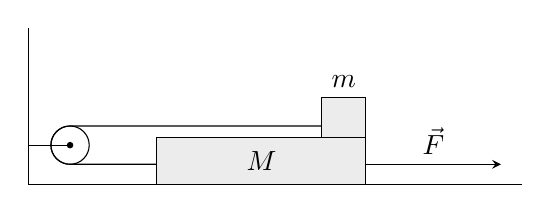
\begin{tikzpicture}[x=.64cm,y=.64cm,>=stealth]
\draw (0,3.1)--(0,0)--(9.8,0);
\draw (0,.78)--(.83,.78);
\draw (.83,.78) circle (.38);
\fill (.83,.78) circle (.065);
\draw (5.82,1.16)--(.83,1.16) arc[start angle=90,end angle=270,radius=.38]--(2.55,.40);
\draw[fill=gray!15] (2.55,0) rectangle (6.7,.94);
\draw[fill=gray!15] (5.82,.94) rectangle (6.7,1.72);
\node at (4.63,.47) {$M$};
\node[above] at (6.26,1.72) {$m$};
\draw[->] (6.7,.40)--(9.38,.40) node[midway,above] {$\vec F$};
\end{tikzpicture}
\end{center}
}{
\smallskip\noindent\textbf{Решение}\par
\textbf{Обоснование}

1. Задачу будем решать в инерциальной системе отсчёта, связанной с поверхностью стола.

2. Тела движутся поступательно, поэтому будем их описывать моделью материальной точки. Следовательно, можно использовать второй закон Ньютона, сформулированный для материальных точек. Силы, действующие на тела, постоянны, поэтому движение бруска и доски равноускоренно.

3. Так как нить нерастяжима, ускорения бруска и доски относительно стола равны по модулю и противоположны по направлению: $|\vec a_1|=|\vec a_2|=a$, $\vec a_1=-\vec a_2$. \hfill(1)

4. Так как блок и нити невесомы и трением в оси блока можно пренебречь, то силы натяжения нити, действующие на доску и брусок, одинаковы: $|\vec T_1|=|\vec T_2|=T$. \hfill(2)

5. Силы трения, действующие на брусок и доску, равны друг другу и противоположны по направлению по третьему закону Ньютона: $\vec F_{\text{тр}1}=-\vec F_{\text{тр}2}$. \hfill(3)

6. Модули сил нормальной реакции доски $\vec N_1$ и давления бруска на доску $\vec P$ также равны друг другу по третьему закону Ньютона: $N_1=P$. \hfill(4)

\textbf{Решение}

1. На рисунке показаны силы, действующие на брусок и на доску. Запишем второй закон Ньютона в проекциях на оси $Ox$ и $Oy$ выбранной системы координат. С учётом (1)–(3) получим:
\[Ma=F-F_{\text{тр}1}-F_{\text{тр}3}-T,\qquad -ma=F_{\text{тр}1}-T,\]
\[N_1=mg,\qquad N_2=Mg+P.\]

\begin{center}
\begin{tikzpicture}[x=.67cm,y=.67cm,>=stealth]
\draw[->] (0,0)--(12.05,0) node[below] {$x$};
\draw[->] (0,0)--(0,3.55) node[left] {$y$};
\node[below left] at (0,0) {$0$};
\draw (0,1.04)--(1.08,1.04);
\draw (1.08,1.04) circle (.50);
\fill (1.08,1.04) circle (.085);
\draw (7.7,1.54)--(1.08,1.54) arc[start angle=90,end angle=270,radius=.50]--(3.4,.54);
\draw[fill=gray!15] (3.4,0) rectangle (8.85,1.2);
\draw[fill=gray!15] (7.7,1.2) rectangle (8.85,2.26);
\draw[->] (8.27,1.73)--(8.27,3.23) node[right] {$\vec N_1$};
\draw[->] (8.27,1.73)--(8.27,.81) node[below right] {$m\vec g$};
\draw[->] (8.27,1.73)--(9.87,1.73) node[right] {$\vec F_{\text{тр}1}$};
\draw[->] (7.7,1.54)--(7.05,1.54) node[above] {$\vec T_1$};
\draw[->] (3.4,.54)--(2.27,.54) node[above] {$\vec T_2$};
\draw[->] (6.1,.64)--(6.1,3.02) node[left] {$\vec N_2$};
\draw[->] (6.1,.64)--(6.1,-1.38) node[right] {$M\vec g$};
\draw[->] (7.48,1.08)--(7.48,.16) node[midway,left] {$\vec P$};
\draw[->] (5.96,.92)--(4.78,.92);
\draw (4.72,1.01)--(3.92,1.60) node[above] {$\vec F_{\text{тр}2}$};
\draw[->] (5.96,.40)--(4.78,.40);
\draw (4.72,.28)--(4.15,-.34) node[below] {$\vec F_{\text{тр}3}$};
\draw[->] (8.85,.54)--(11.13,.54) node[above] {$\vec F$};
\end{tikzpicture}
\end{center}
2. Вычтя второе уравнение из первого, найдём силу, действующую на доску:
\[F=(M+m)a+2F_{\text{тр}1}+F_{\text{тр}3}.\]
3. Далее $F_{\text{тр}1}=\mu_1N_1=\mu_1mg$. С учётом (4) получим $F_{\text{тр}3}=\mu_2N_2=\mu_2(M+m)g$. В итоге:
\[\begin{aligned}F&=(M+m)(a+\mu_2g)+2\mu_1mg\\&=(0{,}8+0{,}2)(1+0{,}3\cdot10)+2\cdot0{,}5\cdot0{,}2\cdot10=6\,\text{Н}.\end{aligned}\]
Ответ: $F=6\,\text{Н}$.
}

% Source 2942: https://phys-ege.sdamgia.ru/problem?id=2942
\BankTask{2942}{
Снаряд массой $4\,\text{кг}$, летящий со скоростью $400\,\text{м/с}$, разрывается на две равные части, одна из которых летит в направлении движения снаряда, а другая — в противоположную сторону. В момент разрыва суммарная кинетическая энергия осколков увеличилась на величину $\Delta E=0{,}5\,\text{МДж}$. Определите скорость осколка, летящего по направлению движения снаряда.
}{
\smallskip\noindent\textbf{Решение}\par
\textbf{Обоснование.}

Задачу будем решать в инерциальной системе отсчета, связанной с Землей. Все тела будем считать материальными точками. Трением снаряда и осколков о воздух пренебрежем.

Для описания разрыва снаряда использован закон сохранения импульса системы тел. Он выполняется в инерциальной системе отсчета, если сумма внешних сил, приложенных к телам системы, равна нулю. В данном случае из-за отсутствия сопротивления воздуха внешней силой является только сила тяжести $m\vec g$, которая не равна нулю. Но этим можно пренебречь, считая время разрыва гранаты малым. За малое время разрыва импульс каждого из осколков меняется на конечную величину за счет больших внутренних сил, разрывающих снаряд при взрыве. По сравнению с этими большими силами конечная сила тяжести пренебрежимо мала. Так как время разрыва гранаты считаем малым, то можно пренебречь и изменением потенциальной энергии гранаты и его осколков в поле тяжести в процессе разрыва. В инерциальной системе отсчета выполняется законы сохранения импульса и энергии с учетом энергии разрыва.

Перейдем к решению.

По закону сохранения импульса тел: $2m\vec v_0=m\vec v_1+m\vec v_2$, где $m$ — масса одного осколка. По закону сохранения энергии для незамкнутой системы: $\Delta E=E_{\text{к}1}+E_{\text{к}2}-E_{\text{к}0}$, где кинетическая энергия осколков после разрыва $E_{\text{к}1}=\frac{mv_1^2}{2}$ и $E_{\text{к}2}=\frac{mv_2^2}{2}$, кинетическая энергия снаряда до взаимодействия $E_{\text{к}0}=\frac{2mv_0^2}{2}$. Проецируя векторную запись на горизонтальную ось, объединяя уравнения, получаем систему уравнений для решения задачи:
\[\begin{cases}2mv_0=mv_1-mv_2,\\\dfrac{2mv_0^2}{2}+\Delta E=\dfrac{mv_1^2}{2}+\dfrac{mv_2^2}{2}.\end{cases}\]
Выразим $v_2$ из первого уравнения: $v_2=v_1-2v_0$ и подставим во второе уравнение. Получим:
\[v_1^2-2v_0v_1+v_0^2-\frac{\Delta E}{m}=0.\]
Отсюда следует: $\Delta E=m(v_1-v_0)^2$. Скорость осколка:
\[v_1=v_0+\sqrt{\frac{\Delta E}{m}}=400+\sqrt{\frac{0{,}5\cdot10^6}{2}}=900\,\text{м/с}.\]
Ответ: $v_1=900\,\text{м/с}$.
}

% Source 38623: https://phys-ege.sdamgia.ru/problem?id=38623
\BankTask{38623}{
В установке, изображённой на рисунке, масса грузика $m$ подобрана так, что первоначально покоящаяся тележка после толчка вправо движется равномерно по поверхности трибометра. С каким ускорением будет двигаться тележка, если её толкнуть влево? Масса грузика $m$ в $9$ раз меньше массы тележки $M$. Блок идеален. Нить невесома и нерастяжима. Силу сопротивления движению тележки считать постоянной и одинаковой в обоих случаях. Обоснуйте применимость законов, используемых для решения задачи.
\begin{center}
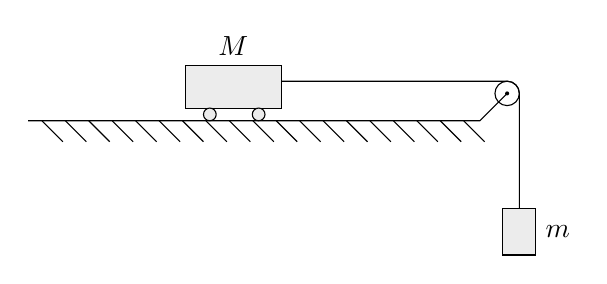
\begin{tikzpicture}[x=.62cm,y=.62cm]
\draw (0,0)--(9.25,0)--(9.81,.56);
\foreach \x in {.28,.76,...,8.96} {\draw (\x,0)--++(.43,-.43);}
\draw (9.81,.56) circle (.25);
\fill (9.81,.56) circle (.042);
\draw (5.18,.81)--(9.81,.81) arc[start angle=90,end angle=0,radius=.25]--(10.06,-1.80);
\draw[fill=gray!15] (3.22,.26) rectangle (5.18,1.13);
\draw[fill=gray!15] (3.72,.13) circle (.13);
\draw[fill=gray!15] (4.72,.13) circle (.13);
\node[above] at (4.2,1.13) {$M$};
\draw[fill=gray!15] (9.72,-1.80) rectangle (10.40,-2.75);
\node[right] at (10.40,-2.275) {$m$};
\end{tikzpicture}
\end{center}
}{
\smallskip\noindent\textbf{Решение}\par
\textbf{Обоснование.}

1. Рассмотрим задачу в системе отсчета, связанной с Землей. Будем считать эту систему отсчета инерциальной (ИСО).

2. Грузик и тележка движутся поступательно, поэтому описываем их моделью материальной точки. В ИСО движение материальной точки описываем вторым законом Ньютона.

3. Нить невесома, блок идеален (масса блока ничтожна, трения нет), поэтому модуль силы натяжения нити в любой ее точке одинаковый.

4. Нить нерастяжима, при прямолинейном поступательном движении модули ускорений грузика и тележки будут одинаковыми.

5. Движение тележки поступательное по шероховатой поверхности, поэтому на нее действует сила трения скольжения.

Перейдем к решению.

В горизонтальном направлении на тележку действуют сила трения и сила натяжения нити. В первом случае силы направлены в разные стороны и компенсируют друг друга, поэтому тележка движется равномерно. Во втором случае они обе направлены против движения, тележка движется равнозамедленно. Запишем для них второй закон Ньютона для тележки и грузика в первом случае:
\[\vec T_1+\vec F_{\text{тр}}=0,\qquad \vec T_1+m\vec g=0.\]
В проекции на оси получаем:
\[T_1-F_{\text{тр}}=0,\qquad T_1-mg=0.\]
Откуда получаем: $F_{\text{тр}}=mg$.

Запишем для них второй закон Ньютона для тележки и грузика во втором случае:
\[\vec T_2+\vec F_{\text{тр}}=M\vec a,\qquad \vec T_2+m\vec g=m\vec a.\]
В проекции на оси получаем:
\[T_2+F_{\text{тр}}=Ma,\qquad mg-T_2=ma.\]
Решая систему уравнений, имеем: $a(M+m)=F_{\text{тр}}+mg=2mg$.

В результате находим ускорение тележки:
\[a=\frac{2mg}{M+m}=\frac{2mg}{m+9m}=\frac g5=\frac{10}{5}=2\,\text{м/с}^2.\]
Ответ: $2\,\text{м/с}^2$.
}

% Source 38860: https://phys-ege.sdamgia.ru/problem?id=38860
\BankTask{38860}{
\begin{center}\begin{tikzpicture}[task graph,>=stealth]\draw(-.82,0)--(4,0);\draw(-.6,0)--(-.6,3.3);\draw[<->](-.6,0)--(-.6,3.3)node[midway,left]{\(H\)};\draw(-.6,3.3)--(0,3.3);\draw[<->](0,0)--(0,1.96)node[midway,left]{\(h\)};\draw[dashed](0,1.96)--(0,3.3);\draw[fill=gray!15](0,3.3)circle(.21);\draw(-.46,2.23)--(.46,1.69);\draw(0,2.33)arc(90:149:.37)node[midway,above left]{\(\alpha\)};\draw[dashed](0,1.96) parabola bend(2.35,3.02)(3.7,2.72);\draw[<->](2.35,0)--(2.35,3.02)node[midway,left]{\(h_1\)};\end{tikzpicture}\end{center}Шарик падает из состояния покоя и на высоте h  =  $1\,\text{м}$ от поверхности Земли абсолютно упруго ударяется о доску, расположенную под углом $\alpha =30 ^\circ$ к горизонту (см. рисунок). Модуль скорости шарика после отскока от доски равен модулю скорости шарика непосредственно перед ударом. После удара шарик поднялся на максимальную высоту h$_{1}$  =  $1{,}25\,\text{м}$ от поверхности Земли. Определите с какой высоты H над поверхностью Земли упал шарик, если после удара его скорость направлена под углом $2 \alpha$ к вертикали. Сопротивлением воздуха пренебречь. 
Обоснуйте применимость используемых законов к решению задачи.
}{
\smallskip\noindent\textbf{Решение}\par
Обоснование
Систему отсчета, связанную с Землей, будем считать инерциальной. Шарик движется поступательно, поэтому его можно принять за материальную точку. По условию задачи силой сопротивления воздуха можно пренебречь. Поэтому шарик движется в поле Земного тяготения. Следовательно, для описания движения тел до столкновения с доской можно использовать закон сохранения энергии
Поскольку при ударе о доску модуль шарика не изменился, то можно считать, что удар абсолютно упругий, следовательно, угол отскока равен углу при падении и равен $\alpha .$
Движение шарика после отскока от доски происходит под действием только силы тяжести, поэтому он движется с ускорением свободного падения.

Перейдем к решению. \begin{center}\begin{tikzpicture}[task graph,>=stealth]\draw(-.82,0)--(1.3,0);\draw(-.6,0)--(-.6,3.3);\draw[<->](-.6,0)--(-.6,3.3)node[midway,left]{\(H\)};\draw(-.6,3.3)--(0,3.3);\draw[<->](0,0)--(0,1.96)node[midway,left]{\(h\)};\draw[dashed](0,1.96)--(0,3.3);\draw[fill=gray!15](0,3.3)circle(.21);\draw(-.46,2.23)--(.46,1.69);\draw(0,2.33)arc(90:149:.37)node[midway,above left]{\(\alpha\)};\draw[->](0,1.96)--(.57,2.84)node[above]{\(\vec n\)};\draw[->](0,1.96)--(1.28,2.54);\draw[dashed](0,1.96)--(1.36,1.96);\draw(1.02,1.96)arc(0:24.4:1.02)node[midway,right]{\(\beta\)};\draw(0,2.54)arc(90:57:.58)node[midway,above right]{\(\alpha\)};\end{tikzpicture}\end{center}
Рассмотрим движение шарика до соударения о доску. В верхней точке он обладал потенциальной энергией $E_{\,\text{п}1}= mgH,$ в момент удара  — потенциальной $E_{\,\text{п}2}= mgh$ и кинетической $E_{\,\text{к}2}= \frac{m v ^2}{2} ,$ где m  — масса шарика, \ensuremath{\upsilon}  — скорость шарика в момент удара о доску. По закону сохранения энергии $E_{\,\text{п}1}=E_{\,\text{п}2} + E_{\,\text{к}2}.$ Тогда получаем:

$mgH=mgh + \frac{m v ^2}{2} ,$
$H=h + \frac{v ^2}{2g} . \qquad ( 1 )$

Из рисунка следует, что угол между скоростью при отскоке и горизонтом равен $\beta =90 ^\circ - 2 \alpha .$
Дальнейшее движение шарика происходило с ускорением свободного падения g. Проекция начальной скорости на вертикальную ось равна $v _y= v \sin \beta = v \sin ( 90 ^\circ - 2 \alpha ) = v \cos 2 \alpha .$ В точке максимального подъема $v_{y1}=0.$ Если выбрать в качестве начального уровня высоты точку отскока, то максимальная высота подъема при равноускоренном движении

\[h_1 - h= \frac{v_{y1} ^2 - v _y ^2}{- 2g} = \frac{v ^2 \cos ^2 2 \alpha}{2g} . \qquad ( 2 )\]

Объединяя формулы ($1$) и ($2$), получаем:

\[H=h + \frac{h_1 - h}{\cos ^2 2 \alpha} =1 + \frac{1{,}25 - 1}{0{,}25} =2\,\text{м}.\]

Ответ: $2\,\text{м}$.
}

% Source 25969: https://phys-ege.sdamgia.ru/problem?id=25969
\BankTask{25969}{
Пружинное ружье наклонено под углом $\alpha =30 ^\circ$ к горизонту. Энергия сжатой пружины равна $0{,}41\,\text{Дж}$. При выстреле шарик массой $m=50\,\text{г}$ проходит по стволу ружья расстояние b, вылетает и падает на расстоянии $L=1\,\text{м}$ от дула ружья в точку M, находящуюся с ним на одной высоте с дулом. (см. рис.). Найдите расстояние b. Трением в стволе и сопротивлением воздуха пренебречь.
Какие законы Вы использовали для описания движения шарика? Обоснуйте их применение к данному случаю.
\begin{center}\begin{tikzpicture}[task graph,>=stealth]\draw(0,0)--(4.6,0);\draw(0,0)--(4.6,2.75)--(10.2,2.75);\draw(0,0)--(-.25,.41)--(4.35,3.16)--(4.6,2.75);\draw[<->](1.2,1.2)--(4.31,3.06)node[midway,above]{\(b\)};\draw[<->](4.6,2.01)--(10.2,2.01)node[midway,below]{\(L\)};\draw(4.6,2.01)--(4.6,2.75)(10.2,2.01)--(10.2,2.75);\foreach \x in {4.7,4.85,...,10.1}{\draw(\x,2.75)--++(-.12,-.12);}\fill(10.2,2.75)circle(1.5pt)node[above right]{\(M\)};\draw(.72,0)arc(0:31:.72)node[midway,right]{\(\alpha\)};\begin{scope}[rotate=31]\draw plot[domain=.1:1.42,samples=120](\x,{.22+.13*sin(2727*\x)});\draw[fill=gray!15](1.63,.22)circle(.21)node[below right,xshift=2pt,yshift=-6pt]{\(m\)};\end{scope}\end{tikzpicture}\end{center}
}{
\smallskip\noindent\textbf{Решение}\par
Обоснование 
Систему отсчета, связанную с Землей, будем считать инерциальной. При движении пули по дулу пистолета на ее действуют силы тяжести, сила упругости и сила реакции опоры, не действуют сила трения (так как дуло можно считать абсолютно гладким) и сила сопротивления воздуха. В ИСО изменение полной механической энергии равно работе всех не потенциальных сил, действующих на тело. В данной задаче такой силой является сила реакции опоры $\vec N.$ Так как в процессе движения по стволу ружья сила реакции опоры $\vec N$ перпендикулярна поверхности, то ее работа равна нулю и $E_{\,\text{мех}}$ сохраняется в ИСО. 
При движении после вылета из трубки мы можем пренебречь действием силы сопротивления воздуха, значит, движение мяча происходит в поле Земного тяготения. Ось 0x направим горизонтально, ось 0y направим вертикально вверх. Тогда проекция вектора ускорения на ось 0x равна $0$, поэтому для описания движения по горизонтали можно использовать законы прямолинейного равномерного движения. Проекция вектора ускорения на ось 0y равна  — g, поэтому для описания движения по вертикали можно использовать законы прямолинейного равноускоренного движения.

Перейдем к решению.
$1$.  Рассмотрим движение шарика внутри трубки. По закону сохранения энергии $E_{\,\text{п}\,\text{пр}}=E_{\,\text{п}\,\text{ш}} + E_{\,\text{к}},$ где $E_{\,\text{п}\,\text{ш}}=mgh,$ $E_{\,\text{к}}= \frac{m v ^2}{2} .$ Откуда получаем:

\[E_{\,\text{пр}}=mgh + \frac{m v ^2}{2} .\]

По рисунку $h=b \cdot \sin \alpha .$
$2$.  Шарик вылетает из трубки со скоростью $v$ под углом $30 ^\circ$ к горизонту. При отсутствии сопротивления воздуха по горизонтальной оси движение равномерное, так как $g_x=0,$ по вертикальной оси, направленной вертикально вверх,  — равноускоренное с ускорением свободного падения, так как $g_y= - g.$ Такое движение описываем уравнениями $s_x= v _xt$ и $s_y= v _yt - \frac{gt ^2}{2} .$ Проекции начальной скорости при вылете из трубки $v _x= v \cos \alpha ,$ $v _y= v \sin \alpha .$ Учитывая, что в момент падения на горизонтальную плоскость $s_y=0,$ находим из приведенных формул время полета шарика: 

\[t= \frac{2 v \sin \alpha}{g} .\]

Тогда дальность полета шарика равна $L= \frac{v ^2 \sin 2 \alpha}{g} .$
$3$.  Объединяя записанные формулы, выразим искомую величину:

\[b= \frac{2E_{\,\text{пр}} \sin 2 \alpha - mgL}{2mg \sin \alpha \sin 2 \alpha} = \frac{2 \cdot 0{,}41 \cdot \sin 60 ^\circ - 0{,}05 \cdot 10 \cdot 1}{2 \cdot 0{,}05 \cdot 10 \cdot 0{,}5 \cdot \sin 60 ^\circ} \approx 0{,}485\,\text{м}=48{,}5\,\text{см}.\]

Ответ: $48{,}5\,\text{см}$.
}

% Source 50800: https://phys-ege.sdamgia.ru/problem?id=50800
\BankTask{50800}{
\begin{center}\begin{tikzpicture}[task graph,>=stealth]\draw(-1.15,3.57)--(1.1,3.57);\foreach \x in {-1.1,-.8,...,1.0}{\draw(\x,3.57)--++(.24,.24);}\draw(0,3.57)--(0,2.18) circle(.75);\draw(-.75,2.18)--(-.75,-.20) (.75,2.18)--(.75,-.83);\draw[fill=gray!15](-1.29,-.96)rectangle(-.21,-.20)node[midway]{\(M\)};\draw[fill=gray!15](.22,-1.59)rectangle(1.28,-.83)node[midway]{\(M\)};\draw[fill=gray!30](.50,-.83)rectangle(1.0,-.38)node[midway,right,xshift=9pt]{\(m\)};\end{tikzpicture}\end{center}Два одинаковых бруска массой M  =  $500\,\text{г}$ связаны между собой невесомой нерастяжимой нитью, перекинутой через невесомый гладкий блок, неподвижно закреплённый на потолке (см. рис.). На один из блоков кладут груз массой m  =  $100\,\text{г}$, и система приходит в движение. С какой силой F груз будет давить на брусок? Сделайте схематический рисунок с указанием сил, действующих на бруски и груз. Обоснуйте применимость законов, используемых для решения задачи.
}{
\smallskip\noindent\textbf{Решение}\par
Обоснование. Cистему отсчета, связанную с Землей, будем считать инерциальной. Так как движение грузов поступательное, то их можно описывать моделью материальной точки. Значит, можно применять законы Ньютона для описания движения грузов. Нить, которая связывает тело массой М и тело массой M + m с перегрузком, является невесомой, а блок  — идеальным (его масса равна нулю, трением в его оси вращения можно пренебречь). Следовательно, на оба тела действует одинаковая по модулю сила натяжения нити. Кроме того, нить нерастяжима. Поэтому оба тела движутся с одинаковым по модулю ускорением.

\begin{center}\begin{tikzpicture}[task graph,>=stealth]\draw(-1.15,3.57)--(1.1,3.57);\foreach \x in {-1.1,-.8,...,1.0}{\draw(\x,3.57)--++(.24,.24);}\draw(0,3.57)--(0,2.18) circle(.75);\draw(-.75,2.18)--(-.75,-.20) (.75,2.18)--(.75,-.83);\draw[fill=gray!15](-.94,-1.07)rectangle(-.56,-.40)(.56,-1.66)rectangle(.94,-.7);\draw[->] (0,2.18)--(0,3.4) node[right]{\(\vec F\)};\draw[->] (0,2.18)--(0,.92) node[right]{\(\vec F\)};\draw[->] (-.75,2.18)--(-.75,.92) node[right]{\(\)};\draw[->] (.75,2.18)--(.75,.92) node[right]{\(\)};\draw[->] (-.75,-.73)--(-.75,.6) node[left]{\(\vec T_1\)};\draw[->] (.75,-1.2)--(.75,.35) node[right]{\(\vec T_2\)};\draw[->] (-.75,-.73)--(-.75,-1.69) node[left]{\(M\vec g\)};\draw[->] (.75,-1.2)--(.75,-2.4) node[right]{\((M+m)\vec g\)};\draw[->] (2.66,3.3)--(2.66,-1.42) node[right]{\(X\)};\end{tikzpicture}\end{center}
Перейдем к решению. Запишем, на основании второго закона Ньютона, уравнения движения для обоих грузов в проекции на вертикальную ось, направленную вниз (см. рис.):

$Ma_1=Mg - T_1,$ $( M + m ) a_2= ( M + m ) g - T_2.$

Здесь через $a_1$ и $a_2$ обозначены проекции ускорений грузов M и $( M + m )$ на вертикальную ось, а через $T_1$ и $T_2$  — проекции сил натяжения нити на ту же ось.
В силу условия задачи из-за нерастяжимости нити $a_1= - a_2= - a,$ а из-за невесомости блока и нити и отсутствия трения$T_1=T_2=T.$ 
Из написанных уравнений получаем: 

\[a= \frac{m}{m + 2M} g.\]

Рассмотрим движение только перегрузка. Он давит на груз силой, которая по третьему закону Ньютона равна $F=N.$ Запишем второй закон Ньютона для перегрузка в проекции на вертикальную ось:

\[mg - N=ma.\]

Тогда сила, с которой перегруз давит на груз при их движении, равна:

\[F=m ( g - a ) = \frac{2mMg}{m + 2M} = \frac{2 \cdot 10 \cdot 0{,}1 \cdot 0{,}5}{0{,}1 + 2 \cdot 0{,}5} \approx 0{,}91\,\text{Н}.\]

Ответ: $\approx 0{,}91\,\text{Н}.$
}

% Source 29761: https://phys-ege.sdamgia.ru/problem?id=29761
\BankTask{29761}{
На горизонтальной поверхности неподвижно закреплена абсолютно гладкая полусфера радиусом $R=2{,}5$ м. С ее верхней точки из состояния покоя соскальзывает маленькое тело. В некоторой точке тело отрывается от сферы и летит свободно. Найдите скорость тела в момент отрыва от сферы. Сопротивлением воздуха пренебречь. Обоснуйте применимость используемых законов к решению задачи.
}{
\smallskip\noindent\textbf{Решение}\par
Обоснование
Систему отсчета, связанную с Землей, будем считать инерциальной. Поскольку размеры тела, соскальзывающего с полусферы, малы, то его можно считать материальной точкой. При движении тела от вершины полусферы выполняется закон сохранения механической энергии, так как полусфера гладкая, и работа силы реакции опоры равна нулю (эта сила перпендикулярна скорости тела). В момент отрыва обращается в ноль сила реакции опоры $\vec N .$ Второй закон Ньютона выполняется в ИСО для модели материальной точки.

Перейдем к решению.
$1$.  Рассмотрим два состояния системы  — в верхней точке полусферы и в точке отрыва от поверхности. В верхней точке шарик обладает потенциальной энергией $E_{p1}=m g h_1,$ причем $h_1=R.$ В точке отрыва от поверхности шарик обладает кинетической энергией $E_{k2}= \frac{m v ^2}{2}$ и потенциальной энергией $E_{p2}=m g h.$ Шарик при движении не вращается вследствие отсутствия силы трения, поэтому кинетической энергией вращения можно пренебречь.
По закону сохранения энергии:

\[m g R= \frac{m v ^2}{2} + m g h.\]

$2$.  Шарик отрывается от поверхности полусферы в том случае, когда сила реакции опоры становится равной нулю. На шарик действует сила тяжести, при движении по окружности ускорение направлено к центру окружности. Тогда по второму закону Ньютона в проекции на ось, совпадающую с вектором ускорения, получаем: $m a=m g \cos \alpha .$ Из рисунка видно, что $\cos \alpha = \frac{h}{R} .$ \begin{center}\begin{tikzpicture}[task graph,>=stealth]\draw(-2.04,0)--(3.08,0);\draw(1.6,0)arc(0:180:1.6);\draw(0,0)--(0,1.6)node[midway,left]{\(R\)};\filldraw[fill=gray!15](0,1.68)circle(.09) (1.13,1.13)circle(.09);\draw[dashed](0,0)--(1.13,1.13);\draw(1.13,1.13)--(3.08,1.13);\draw[<->](2.82,0)--(2.82,1.13)node[midway,right]{\(h\)};\draw(1.13,.8)arc(270:225:.33)node[midway,below left]{\(\alpha\)};\draw[->] (1.13,1.13)--(.49,.49) node[left]{\(\vec a\)};\draw[->] (1.13,1.13)--(1.13,-.55) node[right]{\(m\vec g\)};\end{tikzpicture}\end{center}
$3$.  При движении по окружности центростремительное ускорение равно $a= \frac{v ^2}{R} .$ 
$4$.  Объединяя формулы и решая совместно уравнения, выражаем скорость шарика в момент отрыва:

\[v = \sqrt{\frac{2 g R}{3}} = \sqrt{\frac{2 \cdot 10 \cdot 2{,}5}{3}} \approx 4{,}1 \,\text{м/с}.\]

Ответ: $4{,}1\,\text{м/с}$.
}

% Source 25930: https://phys-ege.sdamgia.ru/problem?id=25930
\BankTask{25930}{
\begin{center}\begin{tikzpicture}[task graph,>=stealth]\draw (-1.4,-.4)--(3.2,-.4);\draw[fill=gray!15] (-.65,-.4) rectangle(2.45,0);\draw[double] (0,0)--(2.4,1.4);\draw (.6,0) arc (0:30:.6) node[midway,right]{\(\alpha\)};\draw(2.4,1.4)--(2.33,1.16)--(2.17,1.33)--cycle;\draw(1.6,1.42)--(3.25,1.42);\foreach \x in {1.65,1.85,...,3.05}{\draw (\x,1.42)--++(.15,.15);}\foreach \x in {-1.4,-1.2,...,3}{\draw(\x,-.4)--++(.16,-.16);}\node[above] at(.9,.65){\(m\)};\draw[->] (-.65,-.2)--(-1.85,-.2) node[above]{\(\vec F\)};\draw[->] (-.65,.8)--(-1.85,.8) node[above]{\(\vec v=\mathrm{const}\)};\end{tikzpicture}\end{center}Однородный тонкий стержень массой m = $1\,\text{кг}$ одним концом шарнирно прикреплен к потолку, а другим концом опирается на массивную горизонтальную доску, образуя с ней угол $\alpha$ = $30$°. Под действием горизонтальной силы $\vec F$ доска движется поступательно влево с постоянной скоростью (см. рис.). Стержень при этом неподвижен. Найдите F, если коэффициент трения стержня по доске \ensuremath{\mu} = $0{,}2$. Трением доски по опоре и трением в шарнире пренебречь.
Какие законы Вы используете для описания равновесия системы тел? Обоснуйте их применение к данному случаю.
}{
\smallskip\noindent\textbf{Решение}\par
Обоснование. Систему отсчета, связанную с Землей, будем считать инерциальной. Движение доски поступательное. Следовательно, ее можно принять за материальную точку. В инерциальной системе отсчета для доски, движущейся равномерно, применим второй закон Ньютона. Модуль силы трения $\vec F_{\,\text{тр}1},$ действующей на доску, равен модулю силы трения $\vec F_{\,\text{тр}2},$ действующей на стержень по третьему закону Ньютона. Кроме силы трения на стержень действуют сила реакции опоры, сила реакции шарнира, сила тяжести. Стержень будем считать абсолютно твердым телом (формы и размеры тела неизменны, расстояние между любыми двумя его точками остается неизменным). В инерциальной системе отсчета применимо правило моментов для вращающегося тела. Ось, относительно которой будем рассматривать сумму моментов сил, проведем перпендикулярно плоскости чертежа через точку крепления стержня.

Перейдем к решению.\begin{center}\begin{tikzpicture}[task graph,>=stealth]\draw[->](0,0)--(5,0)node[below]{\(x\)};\draw[->](0,0)--(0,2)node[left]{\(y\)};\node[below left]at(0,0){\(0\)};\draw[fill=gray!15](1.25,.5)rectangle(3.6,.9);\draw[->] (1.25,.7)--(.5,.7) node[above]{\(\vec F\)};\draw[->] (3.6,.7)--(4.35,.7) node[above]{\(\vec F_{\text{тр}1}\)};\end{tikzpicture}\end{center} 
$1$.  В инерциальной системе отсчета Оху, связанной с Землей, доска движется поступательно с постоянной скоростью. Поэтому сумма проекций на ось Ох всех сил, приложенных к доске, равна нулю (рис. а):

\[F_{\,\text{тр}1} - F = 0.\]

$2$.  На рис. б показаны все силы, приложенные к стержню. Силы реакции шарнира представлена горизонтальными и вертикальными составляющими: $\vec T = \vec T_1 + \vec T_2.$ По третьему закону Ньютона $\vec F_{\,\text{тр}2} = - \vec F_{\,\text{тр}1},$ поэтому

\[F_{\,\text{тр}2} = F_{\,\text{тр}1} = F. ( 1 )\]

$3$.  По условию задачи стержень покоится, поэтому сумма моментов сил относительно оси шарнира А равна нулю. Обозначив длину стержня через L, запишем это условие:\begin{center}\begin{tikzpicture}[task graph,>=stealth]\draw[double] (0,0)--(2.4,1.4);\draw (.6,0) arc (0:30:.6) node[midway,right]{\(\alpha\)};\draw[dashed](0,0)--(1.1,0);\node[above left]at(2.4,1.4){\(A\)};\draw[->] (0,0)--(0,.9) node[above]{\(\vec N\)};\draw[->] (0,0)--(-.9,0) node[below]{\(\vec F_{\text{тр}2}\)};\draw[->] (1.2,.7)--(1.2,-.78) node[right]{\(m\vec g\)};\draw[->] (2.4,1.4)--(2.4,2.4) node[above]{\(\vec T_1\)};\draw[->] (2.4,1.4)--(3.2,1.4) node[below]{\(\vec T_2\)};\end{tikzpicture}\end{center}

\[mg \frac{L}{2} \cos \alpha - F_{\,\text{тр}2}L \sin \alpha - NL \cos \alpha = 0. ( 2 )\]

$4$.  Доска движется относительно стержня, поэтому сила трения является силой трения скольжения:

\[F_{\,\text{тр}2} = \mu N. ( 3 )\]

$5$.  Подставив ($3$) в ($2$), получим уравнение

\[mg \cos \alpha - 2\mu N \sin \alpha - 2N \cos \alpha = 0,\]

позволяющее найти реакцию доски:

\[N= \frac{mg}{2 ( 1 + \mu \tan \alpha )} .\]

 Отсюда:

\[F=F_{\,\text{тр}2} = \mu N = \frac{\mu mg}{2 ( 1 + \mu \tan \alpha )} = \frac{0{,}2 \cdot 1 \cdot 10}{2 ( 1 + 0{,}2 \cdot \frac{\sqrt{3}}{3} )} \approx 0{,}9\,\text{Н}.\]

Ответ: $F \approx 0{,}9\,\text{Н}.$
}

% Source 38979: https://phys-ege.sdamgia.ru/problem?id=38979
\BankTask{38979}{
\begin{center}\begin{tikzpicture}[task graph,>=stealth]\draw(-.3,0)--(6,0)--(6,2);\foreach \x in {-.3,-.1,...,5.9}{\draw(\x,0)--++(.15,-.15);}\foreach \y in {.1,.3,...,1.9}{\draw(6,\y)--++(.15,.15);}\draw[fill=gray!15](0,0)rectangle(.6,.58)node[midway]{\(m\)};\draw[fill=gray!15](2,0)rectangle(3.15,1.15)node[midway]{\(M\)};\draw(4.85,0)--(4.85,.9);\draw(4.85,.68)--(4.95,.82)--(5.12,.57)--(5.29,.82)--(5.46,.57)--(5.63,.82)--(5.80,.57)--(6,.82);\node[above]at(5.45,.85){\(k\)};\draw(3.15,0)--(3.15,-.85)(4.85,0)--(4.85,-.85);\draw[<->](3.15,-.58)--(4.85,-.58)node[midway,below]{\(L\)};\draw[->] (.6,.31)--(1.45,.31) node[above]{\(\vec v\)};\end{tikzpicture}\end{center} Небольшое тело массой m  =  $100\,\text{г}$, скользящее по гладкой горизонтальной поверхности, абсолютно неупруго сталкивается с неподвижным телом массой M  =  $2$m. При дальнейшем поступательном движении тела налетают на недеформированную пружину, одним концом прикреплённую к стене (см. рис.). Через какое время t после абсолютно неупругого удара тела вернутся в точку столкновения? Скорость движения тела до столкновения $v = 3 \,\text{м/с}$ жёсткость пружины k  =  $30\,\text{Н/м}$, а расстояние от точки столкновения до пружины L  =  $15\,\text{см}$.
}{
\smallskip\noindent\textbf{Решение}\par
Обоснование.
Рассмотрим решение задачи в системе отсчета, связанной с Землей, которую можно считать инерциальной. Тела движутся поступательно, поэтому их движение можно описывать моделью материальной точки.
При отсутствии силы трения система тел является замкнутой, поэтому в ИСО можем применить закон сохранения импульса тел.
Так как поверхность гладкая, работа внешних сил при движении по горизонтали равна нулю. Поэтому движение брусков до и после касания пружины считаем равномерным. Для тел, составляющих замкнутую систему, можно применить закон сохранения энергии для колебаний пружины. При малой деформации пружины в ИСО колебания пружины с телами считаем гармоническими. 

Перейдем к решению. Для системы тел применим закон сохранения импульса при неупругом ударе: $m \vec v = ( m + M ) \vec u ,$ где u  — скорости тел после неупругого соударения. Учитывая, что $M=2m,$ получаем в проекциях на горизонтальную ось:

$m v =3mu,$ откуда $u= \frac{v}{3} .$

После соударения тела, как единое целое переместятся равномерно на расстояние L до касания с пружиной за время

\[t_1= \frac{L}{u} = \frac{3L}{v} .\]

Далее пружина сначала сожмется до максимальной деформации, а затем распрямится до недеформированного состояния. Время движения тел в этом случае равно $t_2= \frac{T}{2} ,$ где период колебаний пружинного маятника равен $T=2 \pi \sqrt{\frac{m + M}{k}} .$
Таким образом, время движения тел от момента касания до момента отрыва от пружины равно

\[t_2= \pi \sqrt{\frac{3m}{k}} .\]

При отсутствии силы трения по закону сохранения энергии скорость тел в момент отрыва от пружины равна скорости в момент касания u, причем отрыв произойдет в той же точке, где пружина снова станет недеформированной. Поэтому время движения тела вернутся в точку столкновения через промежуток времени t$_{1}$.
В итоге получаем общее время движения тел:

\[t=2t_1 + t_2= \frac{6L}{v} + \pi \sqrt{\frac{3m}{k}} = \frac{6 \cdot 0{,}15}{3} + 3{,}14 \cdot \sqrt{\frac{3 \cdot 0{,}1}{30}} \approx 0{,}614\,\text{с} .\]

Ответ: $t \approx 0{,}614\,\text{с}.$
}

% Source 33076: https://phys-ege.sdamgia.ru/problem?id=33076
\BankTask{33076}{
\begin{center}\begin{tikzpicture}[task graph,>=stealth]\fill[blue!16](0,0)rectangle(2.8,2.8);\draw(0,4.6)--(0,0)--(2.8,0)--(2.8,4.6);\draw(0,2.8)--(2.8,2.8);\draw(-.77,0)--(0,0)(-.77,2.8)--(0,2.8);\draw[<->](-.44,0)--(-.44,2.8)node[midway,left]{\(h\)};\draw[fill=white,fill opacity=.5](0,.14)--(2.61,4.27)--(2.8,4.15)--(.19,.02)--cycle;\end{tikzpicture}\end{center}В гладкий высокий стакан радиусом $4\,\text{см}$ поставили однородную тонкую палочку длиной $10\,\text{см}$ и массой $0{,}9\,\text{г}$, после чего в стакан налили до высоты $4\,\text{см}$ жидкость, плотность которой составляет $0{,}75$ плотности материала палочки. Найдите модуль силы $\vec F,$ с которой верхний конец палочки давит на стенку стакана. Сделайте рисунок с указанием сил, действующих на палочку.
}{
\smallskip\noindent\textbf{Решение}\par
Обоснование. 
$1$.  Выберем систему отсчета, связанную с Землей, будем считать ее инерциальной (ИСО).
$2$.  Палочку будем описывать моделью абсолютно твердого тела (формы и размеры тела неизменны, расстояние между любыми двумя точками тела остаются неизменными).
$3$.  Любое движение твердого тела является суперпозицией поступательного и вращательного движений. Поэтому условий равновесия твердого тела в ИСО ровно два: одно для поступательного движения, другое - для вращательного движения.
$4$.  Сумма приложенных к твердому телу внешних сил равна нулю (условие равновесия твердого тела относительно поступательного движения). Поэтому сумма моментов этих сил относительно любых двух параллельных осей одна и так же. Для удобства выберем ось, проходящую через нижний конец палочки (точку А).
$5$.  Стенки сосуда гладкие (трения нет), поэтому в точке В на палочку со стороны сосуда действует сила $\vec N,$ перпендикулярная стенке.
Перейдем к решению.
\begin{center}\begin{tikzpicture}[task graph,>=stealth]\fill[blue!16](0,0)rectangle(2.8,2.8);\draw(0,4.6)--(0,0)--(2.8,0)--(2.8,4.6);\draw(0,2.8)--(2.8,2.8);\draw(-.77,0)--(0,0)(-.77,2.8)--(0,2.8);\draw[<->](-.44,0)--(-.44,2.8)node[midway,left]{\(h\)};\draw[fill=white,fill opacity=.5](0,.14)--(2.61,4.27)--(2.8,4.15)--(.19,.02)--cycle;\draw(2.8,0)--(3.6,0)(2.8,4.15)--(3.6,4.15);\draw[<->](3.1,0)--(3.1,4.15)node[midway,right]{\(H\)};\draw(.59,0)arc(0:57:.59)node[midway,right]{\(\alpha\)};\draw[->] (2.8,4.15)--(1.48,4.15) node[above]{\(\vec N\)};\draw[->] (.89,1.33)--(.89,2.5) node[left]{\(\vec F_{\mathrm A}\)};\draw[->] (1.39,2.14)--(1.39,.87) node[right]{\(m\vec g\)};\draw[->] (0,0)--(0,.95) node[above right]{\(\vec F_2\)};\draw[->] (0,0)--(.95,0) node[below]{\(\vec F_1\)};\end{tikzpicture}\end{center}
Изобразим силы, действующие на палочку.
Высота конца палочки относительно дна стакана 

\[H= \sqrt{l ^2 - 4R ^2} = \sqrt{0{,}1 ^2 - 4 \cdot 0{,}0016} =0{,}06\,\text{м}.\]

На палочку со стороны воды действует сила Архимеда. Определим объем погруженной части палочки, учитывая, что ее сечение одинаково по всей длине:

$\frac{V_{\,\text{пчт}}}{V} = \frac{h}{H} ,$ откуда $V_{\,\text{пчт}}= \frac{hV}{H} .$

Тогда сила Архимеда равна

\[F_A=\rho_{\,\text{ж}}gV_{\,\text{пчт}}= \frac{\rho_{\,\text{ж}}ghV}{H} = \frac{0{,}75\rho gVh}{H} = \frac{0{,}75mgh}{H} .\]

Запишем правило моментов приложенных сил относительно нижнего конца палочки:

\[mgR - F_{\,\text{А}} \cdot \frac{h}{2} \ctg \alpha - NH=0 .\]

Учитывая, что $\ctg \alpha = \frac{2R}{H} ,$ получаем:

\[mgR - \frac{0{,}75mgh}{H} \cdot \frac{h}{2} \cdot \frac{2R}{H} - NH=0.\]

Откуда сила реакции опоры равна

\[N= \frac{mgR}{H} \cdot ( 1 - 0{,}75 ( \frac{h}{H} ) ^2 ) = \frac{9 \cdot 10 ^{ - 4 } \cdot 10 \cdot 0{,}04}{0{,}06} \cdot ( 1 - 0{,}75 ( \frac{0{,}04}{0{,}06} ) ^2 ) =4\,\text{мН}.\]

По третьему закону Ньютона $F=N=4\,\text{мН}.$

Ответ: $4$ мН.
}

% Source 25739: https://phys-ege.sdamgia.ru/problem?id=25739
\BankTask{25739}{
Внутрь сферической поверхности помещена гантель. Масса большого шарика M = $60\,\text{г}$. Стержень, соединяющий шарики, невесом. Коэффициент трения между большим шариком и сферической поверхностью $0{,}4$. Трение между маленьким шариком и сферической поверхностью отсутствует. Определите, при каком значении массы шарика m гантель будет оставаться в неподвижном состоянии. Считать размеры шариков значительно меньшими, чем размер всей гантели.
Какие законы Вы используете для описания равновесия штанги? Обоснуйте их применение к данному случаю.
\begin{center}\begin{tikzpicture}[task graph,>=stealth]\draw[very thick] (-2.4,1.2)--(-.92,1.2) arc (128:412:1.5)--(2.4,1.2);\draw[dashed] (-1.5,0)--(1.5,0) (0,0)--(0,-1.35);\draw (0,-1.33)--(1.47,0);\draw[fill=gray!15] (0,-1.33) circle(.17) (1.47,0) circle(.08);\node[above] at(-.6,0){\(R\)};\node[above left] at(0,-1.33){\(M\)};\node[above left] at(1.5,0){\(m\)};\end{tikzpicture}\end{center}
}{
\smallskip\noindent\textbf{Решение}\par
Обоснование. Систему отсчета, связанную с Землей, будем считать инерциальной. Каждый из шариков штанги может двигаться поступательно, поэтому их можно считать материальными точками. На них действуют сила тяжести, сила реакции опоры, сила упругости стержня, сила трения. Так как стержень жесткий, то силы реакции, действующие на каждый шарик, равны по модулю $T_1 =T_2=T.$ Для описания поведения шариков в инерциальной системе отсчета можно применить второй закон Ньютона. В данных условиях равнодействующая сил тяжести, реакции опоры и натяжения стержня должна быть меньше силы трения, чтобы шарики оставались в покое.
Перейдем к решению. Изобразим силы, действующие на шарики:
\begin{center}\begin{tikzpicture}[task graph,>=stealth]\draw[very thick] (-2.4,1.2)--(-.92,1.2) arc (128:412:1.5)--(2.4,1.2);\draw[dashed] (-1.5,0)--(1.5,0) (0,0)--(0,-1.35);\draw (0,-1.33)--(1.47,0);\draw[fill=gray!15] (0,-1.33) circle(.17) (1.47,0) circle(.08);\draw[->] (1.47,0)--(.65,0) node[above]{\(\vec N_1\)};\draw[->] (1.47,0)--(2.12,.6) node[right]{\(\vec T_1\)};\draw[->] (1.47,0)--(1.47,-1.05) node[right]{\(m\vec g\)};\draw[->] (0,-1.33)--(0,-.33) node[left]{\(\vec N_2\)};\draw[->] (0,-1.33)--(.70,-1.33) node[above]{\(\vec F_{\text{тр}}\)};\draw[->] (0,-1.33)--(-.7,-1.94) node[left]{\(\vec T_2\)};\draw[->] (0,-1.33)--(0,-2.23) node[right]{\(M\vec g\)};\end{tikzpicture}\end{center}
 По второму закону Ньютона в равновесии суммы сил, действующих на гантель, равны нулю. В проекциях на горизонтальную и вертикальную оси получаем

0х: $N_1 - F_{\,\text{тр}}=0$
Oy: $N_2 - Mg - mg=0$

Тогда $N_1=F_{\,\text{тр}} \leq \mu N_2,$ $N_2= ( M + m ) g,$ следовательно, $N_1 \leq \mu g ( M + m ) .$
Запишем правило моментов приложенных сил относительно оси, проходящей через нижнюю точку:

\[N_1l \sin \alpha - mgl \cos \alpha =0.\]

Учитывая, что $\alpha =45 ^\circ ,$ получаем: $N_1=mg.$
В результате имеем:

\[mg \leq \mu g ( M + m ) ,\]

откуда находим массу верхнего шарика:

\[m \leq \frac{\mu M}{1 - \mu} = \frac{60 \cdot 0{,}4}{1 - 0{,}4} =40\,\text{г}.\]

Ответ: $m \leq 40\,\text{г}.$

Приведем другое решение.
Запишем правило моментов приложенных сил относительно точки O, центра окружности: $mgR = F_{\,\text{тр}} R.$
Из условия равновесия невращающегося твердого тела в проекции на вертикальную ось Oy: $N_2 - Mg - mg = 0.$
Объединяя уравнения и учитывая, что сила трения $F_{\,\text{тр}} \leq \mu N_2,$ получаем:

$N_2 = ( m + M ) g,$
$mg = F_{\,\text{тр}},$
$mg \leq ( m + M ) g \cdot \mu,$
$m \leq \frac{\mu M}{1 - \mu} = \frac{60 \cdot 0{,}4}{0{,}6} = 40 \,\text{г}.$
}

% Source 35186: https://phys-ege.sdamgia.ru/problem?id=35186
\BankTask{35186}{
\begin{center}\begin{tikzpicture}[task graph,>=stealth]\draw(0,0)--(5,0)--(5,2)--cycle;\draw(.72,0)arc(0:21.8:.72)node[midway,right]{\(\alpha\)};\draw(1.96,1.24)circle(.42);\fill(1.96,1.24)circle(1.2pt);\draw(1.80,1.63)--(3.5,2.31);\draw(3.5,1.96)--(3.5,2.69);\foreach \y in {2,2.12,...,2.66}{\draw(3.5,\y)--++(.14,-.12);}\draw(1.96,1.24)--(2.38,1.24)node[right]{\(R\)};\end{tikzpicture}\end{center} На шероховатой наклонной плоскости покоится цилиндр. К верхней части цилиндра по касательной прикреплена параллельная наклонной плоскости невесомая нерастяжимая нить, другой конец которой закреплен на вертикальной стене. Масса цилиндра $1\,\text{кг}$, радиус его основания $20\,\text{см}$, коэффициент трения цилиндра о наклонную плоскость $0{,}5$. Определить предельный угол альфа, при котором цилиндр будет находиться в равновесии. Какие законы Вы используете для решения задачи? Обоснуйте их применение.
}{
\smallskip\noindent\textbf{Решение}\par
\begin{center}\begin{tikzpicture}[task graph,>=stealth]\draw(0,0)--(5,0)--(5,2)--cycle;\draw(.72,0)arc(0:21.8:.72)node[midway,right]{\(\alpha\)};\draw(1.96,1.24)circle(.42);\fill(1.96,1.24)circle(1.2pt);\draw(1.80,1.63)--(3.5,2.31);\begin{scope}[shift={(3.7,2.39)},rotate=21.8]\draw[fill=gray!15](-.22,-.22)rectangle(.22,.22);\end{scope}\node[below right]at(2.12,.85){\(A\)};\draw[->] (1.96,1.24)--(1.20,2.17) node[left]{\(\vec N\)};\draw[->] (1.80,1.63)--(3.02,2.12) node[above]{\(\vec T\)};\draw[->] (2.12,.85)--(3.29,1.32) node[below]{\(\vec F_{\text{тр}}\)};\draw[->] (1.96,1.24)--(1.96,.15) node[right]{\(m\vec g\)};\end{tikzpicture}\end{center}Обоснование. $1$.  Рассмотрим задачу в системе отсчета, связанной с Землей. Будем считать эту систему отсчета инерциальной (ИСО).
$2$.  Описываем цилиндр моделью твердого тела (форма и размеры тела неизменны, расстояние между двумя точками тела остается неизменным ).
$3$.  Любое движение твердого тела является суперпозицией поступательного и вращательного движений. Поэтому условий равновесия твердого тела в ИСО ровно два: одно −для поступательного движения, другое − для вращательного движения.
$4$.  В качестве оси, относительно которой будем считать сумму моментов сил, действующих на цилиндр, выберем ось, проходящую перпендикулярно плоскости рисунка через точку касания цилиндра плоскости А.
$5$.  Нить невесома, поэтому модуль силы натяжения нити в любой ее точке один и тот же.
$6$.  Между цилиндром и поверхностью наклонной плоскости действует сила трения, которая в предельном случае равна $F_{\,\text{тр}}=\mu N.$
Перейдем к решению. Изобразим все силы, действующие на цилиндр: сила тяжести mg, сила реакции опоры N, сила трения F$_{\,\text{тр}}$, сила натяжения нити Т.
Запишем правило моментов относительно точки А:

\[mg \sin \alpha \cdot R - T \cdot 2R=0.\]

Тогда получаем, что $T= \frac{mg \sin \alpha}{2} .$
Применим второй закон Ньютона, учитывая, что ускорение равно $0$:

\[\vec N + \vec T + m\vec g + \vec F_{\,\text{тр}}=0.\]

Найдем проекцию на оси:

$Ox:T + F_{\,\text{тр}} - mg \sin \alpha =0;$
$Oy:N - mg \cos \alpha =0.$

Учитывая, что в предельном случае сила трения равна $F_{\,\text{тр}}=\mu N,$ получаем:

\[T + \mu mg \cos \alpha - mg \sin \alpha =0.\]

Объединяя уравнения, получаем:

\[2\mu \cos \alpha = \sin \alpha .\]

Откуда находим предельный угол наклона плоскости

\[\alpha = \arctan 2\mu= \arctan ( 2 \cdot 0{,}5 ) =45 ^\circ .\]

Данный угол действительно будет максимальным, поскольку при увеличении угла наклона сила трения уменьшится, горизонтальная составляющая силы тяжести увеличится, сила натяжения нити увеличится, в результате чего равновесие нарушится.

Ответ: $45$°.
}

\end{document}
